\documentclass[aspectratio=169,10pt]{beamer}

% --- Pacchetti di base ---
\usepackage{amsmath,amssymb}
\usepackage{booktabs}
\usepackage{tabularx}
\usepackage{adjustbox}
\usepackage{graphicx}
\usepackage{subcaption}
\usepackage{qrcode}
\usepackage{tikz}
\usetikzlibrary{arrows.meta,backgrounds,calc,positioning,shapes.multipart}
\usepackage[edges]{forest}

% --- Stile Forest per i Concrete Syntax Trees (Slide 4) ---
\forestset{
  cst tree/.style={
    for tree={
      l=0cm,
      l sep=0.3cm,
      inner sep=0.05cm,
      s sep=0.2cm,
      font=\fontsize{11.5}{13.0}\selectfont\ttfamily,
    }
  }
}

% --- Colori Personalizzati (Palette Bicocca & Cookie Theme) ---
\definecolor{cookieDemoBlue}{HTML}{356AE6}
\definecolor{unimibBlue}{HTML}{0B3C68}
\definecolor{unimibRed}{HTML}{990000}
\definecolor{techAccent}{HTML}{1A5276}
\definecolor{cardBg}{HTML}{F8FAFC}
\definecolor{metricGreen}{HTML}{1E8449}
\colorlet{WHITE}{white}
\colorlet{BLACK}{black}

% --- Tema Cookie ---
\usetheme[
  accent=cookieDemoBlue,
  progressbar=foot,
  sectionpage=progressbar,
  numbering=fraction,
  numberrail=section,
  block=fill,
  toc=none,
]{cookie}

% --- Regolazione Dimensioni Font Titoli e Struttura ---
\setbeamerfont{frametitle}{size=\fontsize{13}{16}\selectfont,series=\bfseries}
\setbeamerfont{number rail}{size=\fontsize{13}{16}\selectfont,series=\bfseries}
\setbeamerfont{cookie kicker}{size=\scriptsize,series=\bfseries}

% --- Eredità coerente dei font nelle liste (evita cambi arbitrari nei sottoelenchi) ---
\setbeamerfont{itemize/enumerate body}{size=\relax}
\setbeamerfont{itemize/enumerate subbody}{size=\relax}
\setbeamerfont{itemize/enumerate subsubbody}{size=\relax}

% --- Margini compatti per sfruttare al meglio lo spazio orizzontale ---
\setbeamersize{text margin left=0.055\paperwidth, text margin right=0.045\paperwidth}

% --- Rientro compatto e uniforme per elenchi puntati e numerati ---
\setlength{\leftmargini}{1.1em}
\setlength{\leftmarginii}{1.0em}
\setlength{\leftmarginiii}{1.0em}
\setbeamertemplate{itemize/enumerate body begin}{\setlength{\leftmargini}{1.1em}}
\setbeamertemplate{itemize/enumerate subbody begin}{\setlength{\leftmarginii}{1.0em}}

% --- Metadati Presentazione ---
\title[OmniDeps]{A Language-Agnostic Framework\\ for Dependency Extraction}
\subtitle{Master's Thesis in Computer Science}
\author[C. Ferrario]{Christian Ferrario}
\institute{University of Milano-Bicocca}
\date{A.Y. 2025--2026}

% ==============================================================================
% TEMPLATE PER IL FRONTESPIZIO (Slide 1)
% Integrato con lo stile nativo di Cookie Beamer e la gerarchia tipografica
% ==============================================================================
\setbeamertemplate{title page}{%
  \begin{tikzpicture}[remember picture,overlay]
    % Cuneo diagonale nativo Cookie
    \coordinate (cuttop) at ($(current page.north east)+(-0.31\paperwidth,0)$);
    \coordinate (cutbottom) at ($(current page.south east)+(-0.43\paperwidth,0)$);
    \fill[cookieAccent] (cuttop) -- (current page.north east) -- (current page.south east) -- (cutbottom) -- cycle;
    % Badge istituzionale con Logo Bicocca nel cuneo
    \node[anchor=center,fill=white,rounded corners=6pt,inner sep=10pt,draw=cookieLine!40,line width=0.6pt]
      at ($(current page.east)+(-0.16\paperwidth,0)$) {
        
\includegraphics[width=0.20\paperwidth,keepaspectratio]{../images/logo_unimib.pdf}
      };
  \end{tikzpicture}%
  % Colonna testuale sinistra in stile nativo Cookie (.58\paperwidth)
  \vspace*{0.02\paperheight}%
  \begin{minipage}[t]{0.56\paperwidth}
    \raggedright
    \cookiekicker{UNIVERSITÀ DEGLI STUDI DI MILANO-BICOCCA}\par\vspace{0.2em}
    {\footnotesize\color{cookieMuted}Dipartimento di Informatica, Sistemistica e Comunicazione\par}
    \vspace{0.85em}
    {\fontsize{22}{26}\selectfont\bfseries A Language-Agnostic\\Framework for Dependency\\Extraction\par}
    \vspace{0.55em}
    {\small\color{cookieMuted}Master's Thesis in Computer Science\par}
    \vspace{0.75em}
    {\color{cookieAccent}\rule{0.16\paperwidth}{1.4pt}}\par
    \vspace{0.85em}
    \begin{columns}[t,onlytextwidth]
      \column{0.46\linewidth}
        {\scriptsize\color{cookieMuted}Candidate\par}\vspace{0.15em}
        {\normalsize\bfseries Christian Ferrario\par}
        \vspace{0.75em}
        {\scriptsize\color{cookieMuted}Academic Year 2025--2026\par}
      \column{0.52\linewidth}
        {\scriptsize\color{cookieMuted}Supervisors\par}\vspace{0.15em}
        {\small\textbf{Prof. Francesca Arcelli Fontana}}\par\vspace{0.1em}
        {\small\textbf{Dr. Francesco Refolli}\par}
    \end{columns}
  \end{minipage}%
}

\begin{document}

% ==============================================================================
% FRONTESPIZIO & ROADMAP (Cookie nativo via \maketitle e toc=aftertitle)
% ==============================================================================
\maketitle

% ==============================================================================
% SEZIONE 1: CONTESTO E MOTIVAZIONE
% ==============================================================================
\section{Context \& Motivation}

% ==============================================================================
% SLIDE 2: CONTESTO & MOTIVAZIONE
% ==============================================================================
\begin{frame}{Context: Software Evolution \& Dependency Analysis}{Technical Debt and the Role of Dependency Graphs}
  \begin{columns}[T,onlytextwidth]
    \column{0.48\textwidth}
      \cookiekicker{Evolution \& Decay}\par\vspace{0.15em}
      {\small\textbf{Architectural Technical Debt}\par
      Continuous changes degrade system architecture and accumulate structural debt over time.\par}
      \vspace{0.65em}

      \cookiekicker{The Polyglot Reality}\par\vspace{0.15em}
      {\small\textbf{Heterogeneous Systems}\par
      Production codebases routinely combine multiple languages and runtime environments.\par}
      \vspace{0.65em}

      \cookiekicker{The Essential Need}\par\vspace{0.15em}
      {\small\textbf{Structural Visibility}\par
      Reliable dependency graphs are required to detect decay and govern system architecture.\par}

    \column{0.48\textwidth}
      \begin{cookiecard}[title={Why Dependency Graphs?}]
        \footnotesize
        \textbf{Detect Architectural Smells}\par
        Uncover cyclic dependencies, unstable interfaces, and modular erosion beyond single-file scope.\par\vspace{0.5em}
        
        \textbf{Safe Refactoring \& Impact Analysis}\par
        Trace change blast radius and ripple effects before altering critical components.\par\vspace{0.5em}
        
        \textbf{System Comprehension}\par
        Provide an accurate structural map to navigate and understand complex codebases.\par
      \end{cookiecard}
  \end{columns}
\end{frame}

% ==============================================================================
% SLIDE 3: STATO DELL'ARTE & FRAMMENTAZIONE
% ==============================================================================
\begin{frame}{State of the Art: Tooling Fragmentation}{The Cost of Language-Specific Analysis Pipelines}
  \begin{columns}[c,onlytextwidth]
    \column{0.48\textwidth}
      \cookiekicker{Compiler Coupling}\par\vspace{0.15em}
      {\small\textbf{Tied to Native Front-Ends}\par
      Existing analyzers depend on specific compiler internals (\texttt{javac}, Clang, JVM), forcing pipelines to be rebuilt for each language.\par}
      \vspace{0.65em}

      \cookiekicker{Engineering Burden}\par\vspace{0.15em}
      {\small\textbf{The $M \times N$ Proliferation}\par
      Supporting multiple languages requires bundling heterogeneous toolchains, leading to duplicated engineering and tool fragmentation.\par}
      \vspace{0.65em}

      \cookiekicker{The Core Goal}\par\vspace{0.15em}
      {\small\textbf{Decoupled Analysis Pipeline}\par
      Replace language-specific pipelines with a single unified extraction flow.\par}

    \column{0.48\textwidth}
      \centering
      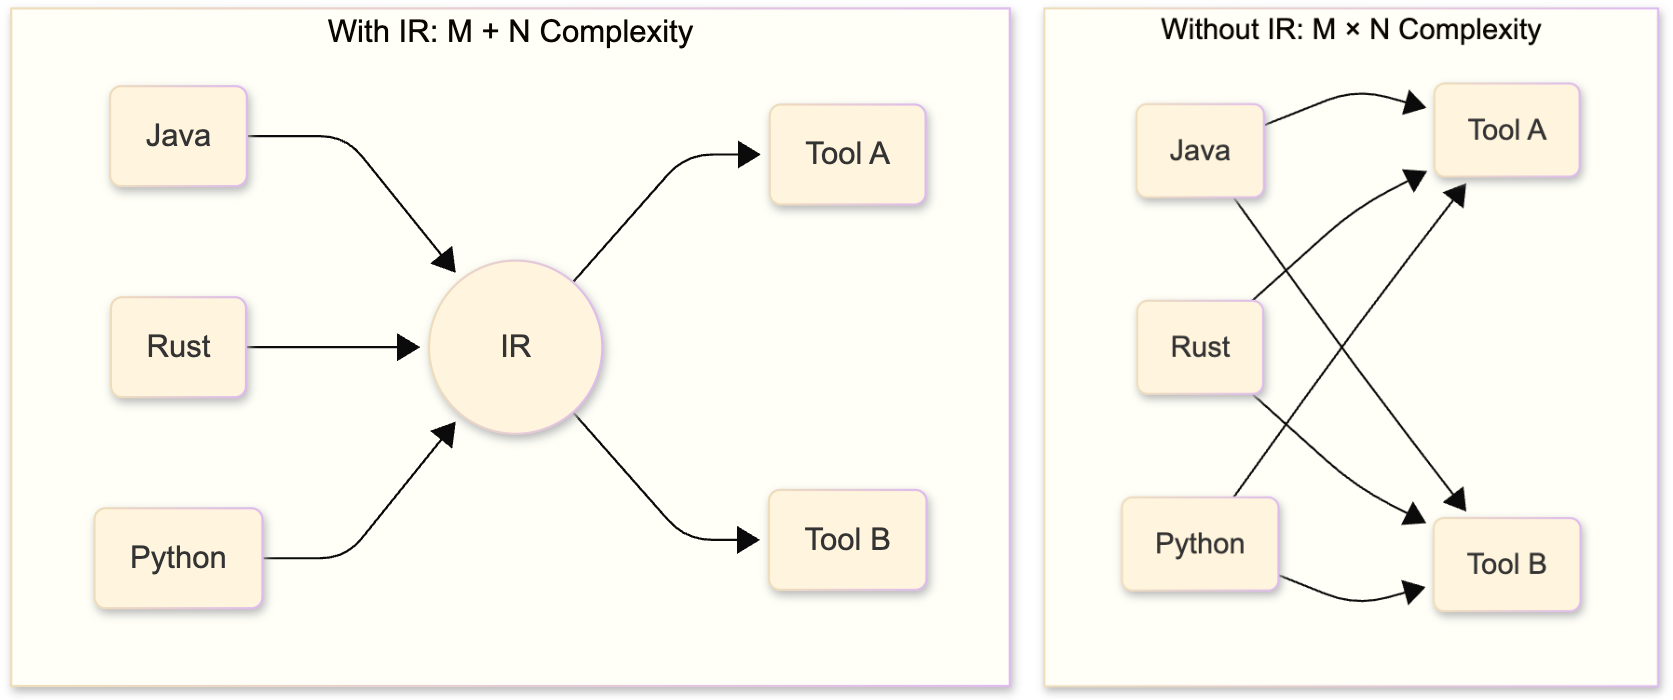
\includegraphics[width=\linewidth,height=0.46\textheight,keepaspectratio]{../images/background/mxn_problem.png}
      \vspace{0.2em}
      \captionof{figure}{\scriptsize\color{cookieMuted}Tool proliferation ($M \times N$) vs. unified intermediate representation ($M + N$).}
  \end{columns}
\end{frame}

% ==============================================================================
% SLIDE 4: L'INTUIZIONE DEI CST
% ==============================================================================
\begin{frame}{Structural Convergence of Syntax Trees}{Syntactic Homology Across Language Grammars}
  \begin{columns}[c,onlytextwidth]
    \column{0.35\textwidth}
      \cookiekicker{Generic Parsing}\par\vspace{0.15em}
      {\small\textbf{Tree-sitter CSTs}\par
      Generates high-performance concrete syntax trees from formal grammars across modern programming languages.\par}
      \vspace{0.40em}

      \cookiekicker{Structural Convergence}\par\vspace{0.15em}
      {\small\textbf{Syntactic Homology}\par
      Equivalent architectural constructs yield structurally identical syntax subtrees across grammars.\par}
      \vspace{0.40em}
          
      \cookiekicker{Pragmatic Assumption}\par\vspace{0.15em}
      {\small\textbf{Compilation-Ready Code}\par
      Source code compiles; extraction maps dependencies without re-validating compiler types or semantics.\par}

    \column{0.7\textwidth}
      \hspace{5em}{\scriptsize\textbf{(a) Rust CST}}\par
      \centering
      \begin{adjustbox}{max width=\linewidth,max totalheight=0.28\textheight}
        \begin{forest}
          cst tree
          [call\_expression
            [field\_expression
              [field\_expression
                [call\_expression
                  [field\_expression
                    [field\_expression
                      [identifier]
                      [field\_identifier]
                    ]
                    [field\_identifier]
                  ]
                  [argument]
                ]
                [field\_identifier]
              ]
              [field\_identifier]
            ]
            [argument]
          ]
        \end{forest}
      \end{adjustbox}

      \raggedright
      \vspace{0.6em}\hspace{5em}{\scriptsize\textbf{(b) Python CST}}\par
      \centering
      \begin{adjustbox}{max width=\linewidth,max totalheight=0.26\textheight}
        \begin{forest}
          cst tree
          [call
            [attribute
              [attribute
                [call
                  [attribute
                    [attribute
                      [identifier]
                      [identifier]
                    ]
                    [identifier]
                  ]
                  [argument\_list]
                ]
                [identifier]
              ]
              [identifier]
            ]
            [argument\_list]
          ]
        \end{forest}
      \end{adjustbox}

      {\par\vspace{1em}\scriptsize\color{cookieMuted}Structural convergence across languages for the code \texttt{a.b.c().d.e()}.\par}
  \end{columns}
\end{frame}

% ==============================================================================
% SLIDE 5: OBIETTIVI E OMNIDEPS
% ==============================================================================
\begin{frame}{Research Objectives \& OmniDeps Proposal}{Design Principles and Evaluation Targets}
  \centering
  {\small Design, formalize, and implement \textbf{OmniDeps}: an extensible, language-agnostic static analysis framework for extracting architectural dependency graphs.}\par\vspace{0.4em}

  \begin{columns}[T,onlytextwidth]
    \column{0.32\textwidth}
      \begin{cookiecard}[title={Pipeline Formalization},height=3.10cm]
        \footnotesize
        \textbf{Functional Staging}\par
        Rigorous 3-phase model guaranteeing sound, type-safe execution.\par\vspace{0.45em}
        \textbf{Universal IR}\par
        Algebraic data types abstracting language-specific syntax.\par
      \end{cookiecard}

    \column{0.32\textwidth}
      \begin{cookiecard}[title={Rust Implementation},height=3.10cm]
        \footnotesize
        \textbf{Decoupled Engine}\par
        Standalone Rust engine operating without native compiler toolchains.\par\vspace{0.45em}
        \textbf{Query Algebra}\par
        Symbol resolution driven by formal scope navigation.\par
      \end{cookiecard}

    \column{0.32\textwidth}
      \begin{cookiecard}[title={Empirical Evaluation},height=3.10cm]
        \footnotesize
        \textbf{Graph Harmonization}\par
        Formal alignment framework for fair cross-tool comparison.\par\vspace{0.45em}
        \textbf{Large-Scale Benchmark}\par
        Validated on 156 repositories ($\sim$98M LOC) against SOTA tools.\par
      \end{cookiecard}
  \end{columns}

  \vspace{0.55em}
  \cookiebadge{Java} \hspace{0.2em}
  \cookiebadge{C / C++} \hspace{0.2em}
  \cookiebadge{Python} \hspace{0.2em}
  \cookiebadge{Rust} \hspace{0.6em}
  {\scriptsize\color{cookieMuted}Diverse paradigms evaluated to validate language-agnostic extensibility\par}
\end{frame}

% ==============================================================================
% SEZIONE 2: ARCHITETTURA DEL FRAMEWORK OMNIDEPS
% ==============================================================================
\section{The Framework}

% ==============================================================================
% SLIDE 6: ARCHITETTURA DELLA PIPELINE
% ==============================================================================
\begin{frame}[t]{Analysis Pipeline Overview}{Functional Composition and Type-Safe Staging}
  \vspace{-0.2em}
  \centering
  {\small $\displaystyle \phi : \mathcal{W} \to \mathcal{G}, \qquad \phi = \gamma \circ \rho \circ \varepsilon = \gamma \circ (\rho_{\text{exec}} \circ \rho_{\text{build}}) \circ \varepsilon$}\par
  \vspace{0.5em}

  \centering
  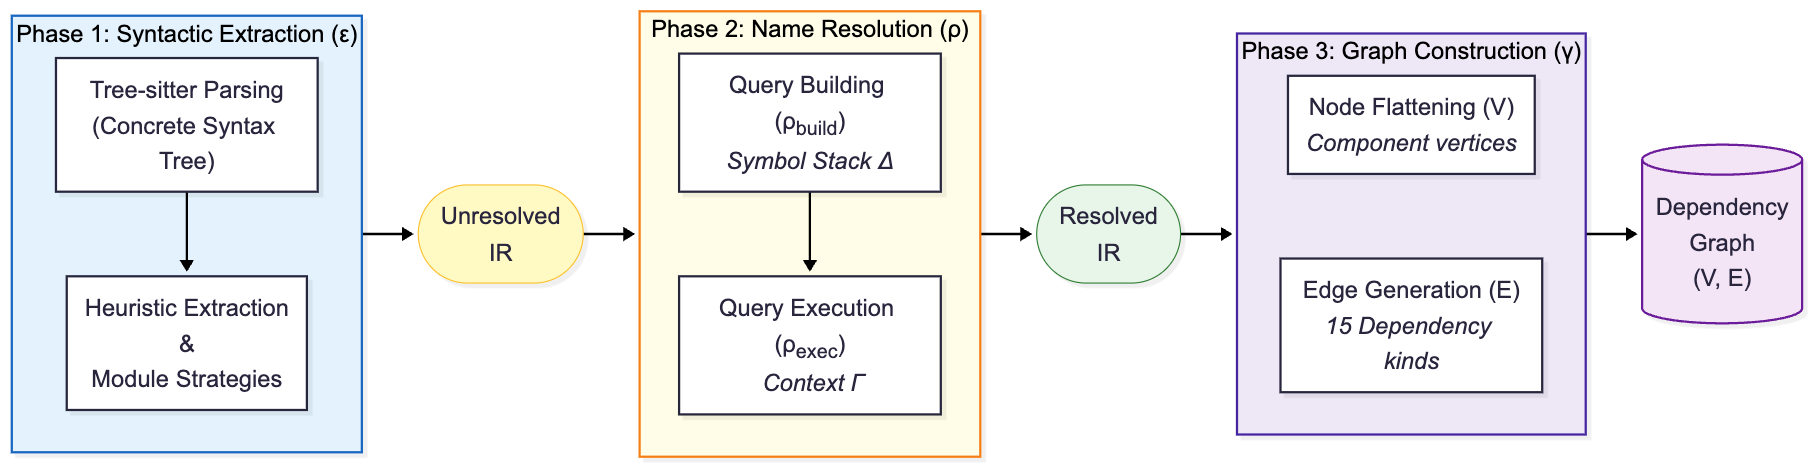
\includegraphics[width=\textwidth,keepaspectratio]{../images/analysis_process/pipeline_detailed.png}

  \begin{columns}[T,onlytextwidth]
    \column{0.32\textwidth}
      \cookiekicker{Phase 1: Extraction}\par\vspace{0.15em}
      {\footnotesize
      \textbf{$\varepsilon : \mathcal{W} \to \mathcal{D}$}\par\vspace{0.1em}
      Parses raw CSTs via Tree-sitter and applies heuristic extraction into unlinked IR. Only phase aware of native syntax.\par
      }

    \column{0.34\textwidth}
      \cookiekicker{Phase 2: Resolution}\par\vspace{0.15em}
      {\footnotesize
      \textbf{$\rho : \mathcal{D} \to \mathcal{D}_{\text{res}}$}\par\vspace{0.1em}
      Builds Scope Tree ($\rho_{\text{build}}$) and resolves symbolic identifiers ($\rho_{\text{exec}}$) via algebraic scope climbing.\par
      }

    \column{0.31\textwidth}
      \cookiekicker{Phase 3: Graph Construction}\par\vspace{0.15em}
      {\footnotesize
      \textbf{$\gamma : \mathcal{D}_{\text{res}} \to \mathcal{G}$}\par\vspace{0.1em}
      Flattens resolved entities into component vertices ($V$) and emits directed dependency edges ($E$).\par
      }
  \end{columns}


\end{frame}

% ==============================================================================
% SLIDE 7: FASE 1 - EXTRACTION
% ==============================================================================
\begin{frame}{Phase 1: Syntactic Extraction}{From Concrete Syntax Trees to Intermediate Representation}
  \begin{columns}[T,onlytextwidth]
    \column{0.32\textwidth}
      \cookiekicker{CST Traversal}\par\vspace{0.15em}
      {\footnotesize
      Parses source files with Tree-sitter, systematically navigating the concrete syntax tree to discover candidate nodes.\par
      }

    \column{0.34\textwidth}
      \cookiekicker{Heuristic Recognition}\par\vspace{0.15em}
      {\footnotesize
      Evaluates declarative predicates (positive matches and negative exclusions) on CST nodes to identify architectural constructs.\par
      }

    \column{0.31\textwidth}
      \cookiekicker{IR Instantiation}\par\vspace{0.15em}
      {\footnotesize
      Extracts textual identifiers and signatures directly from source buffers, populating the unlinked Intermediate Representation.\par
      }
  \end{columns}

  \vspace{0.45em}
  \centering
  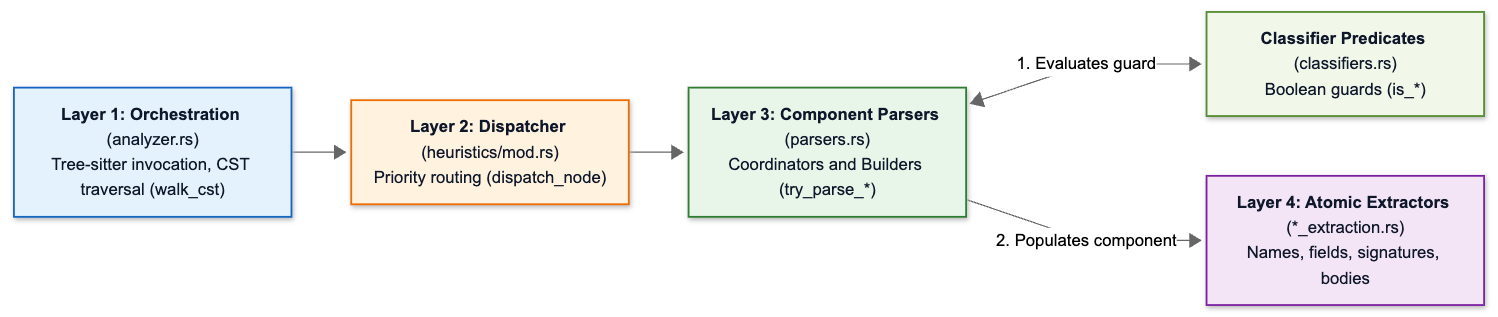
\includegraphics[width=0.96\textwidth,height=0.33\textheight,keepaspectratio]{../images/extraction/extraction_layers.png}
\end{frame}

% ==============================================================================
% SLIDE 8: UNIVERSAL INTERMEDIATE REPRESENTATION
% ==============================================================================
\begin{frame}{Universal Intermediate Representation (IR)}{Hierarchical Domain Model and Language Abstraction}
  \begin{columns}[T,onlytextwidth]
    \column{0.32\textwidth}
      \cookiekicker{Domain Hierarchy}\par\vspace{0.15em}
      {\footnotesize
      Modules nest submodules, types, and functions, faithfully mirroring the logical structure of the codebase.\par
      }

    \column{0.34\textwidth}
      \cookiekicker{Cross-Paradigm Model}\par\vspace{0.15em}
      {\footnotesize
      Unifies OOP, procedural, and systems constructs (classes, structs, traits) into shared algebraic data types.\par
      }

    \column{0.31\textwidth}
      \cookiekicker{Symbolic Placeholders}\par\vspace{0.15em}
      {\footnotesize
      Encapsulates references to external or unlinked symbols as \texttt{TypeRef} variants, deferred to Phase 2.\par
      }
  \end{columns}

  \vspace{0.15em}
  \centering
  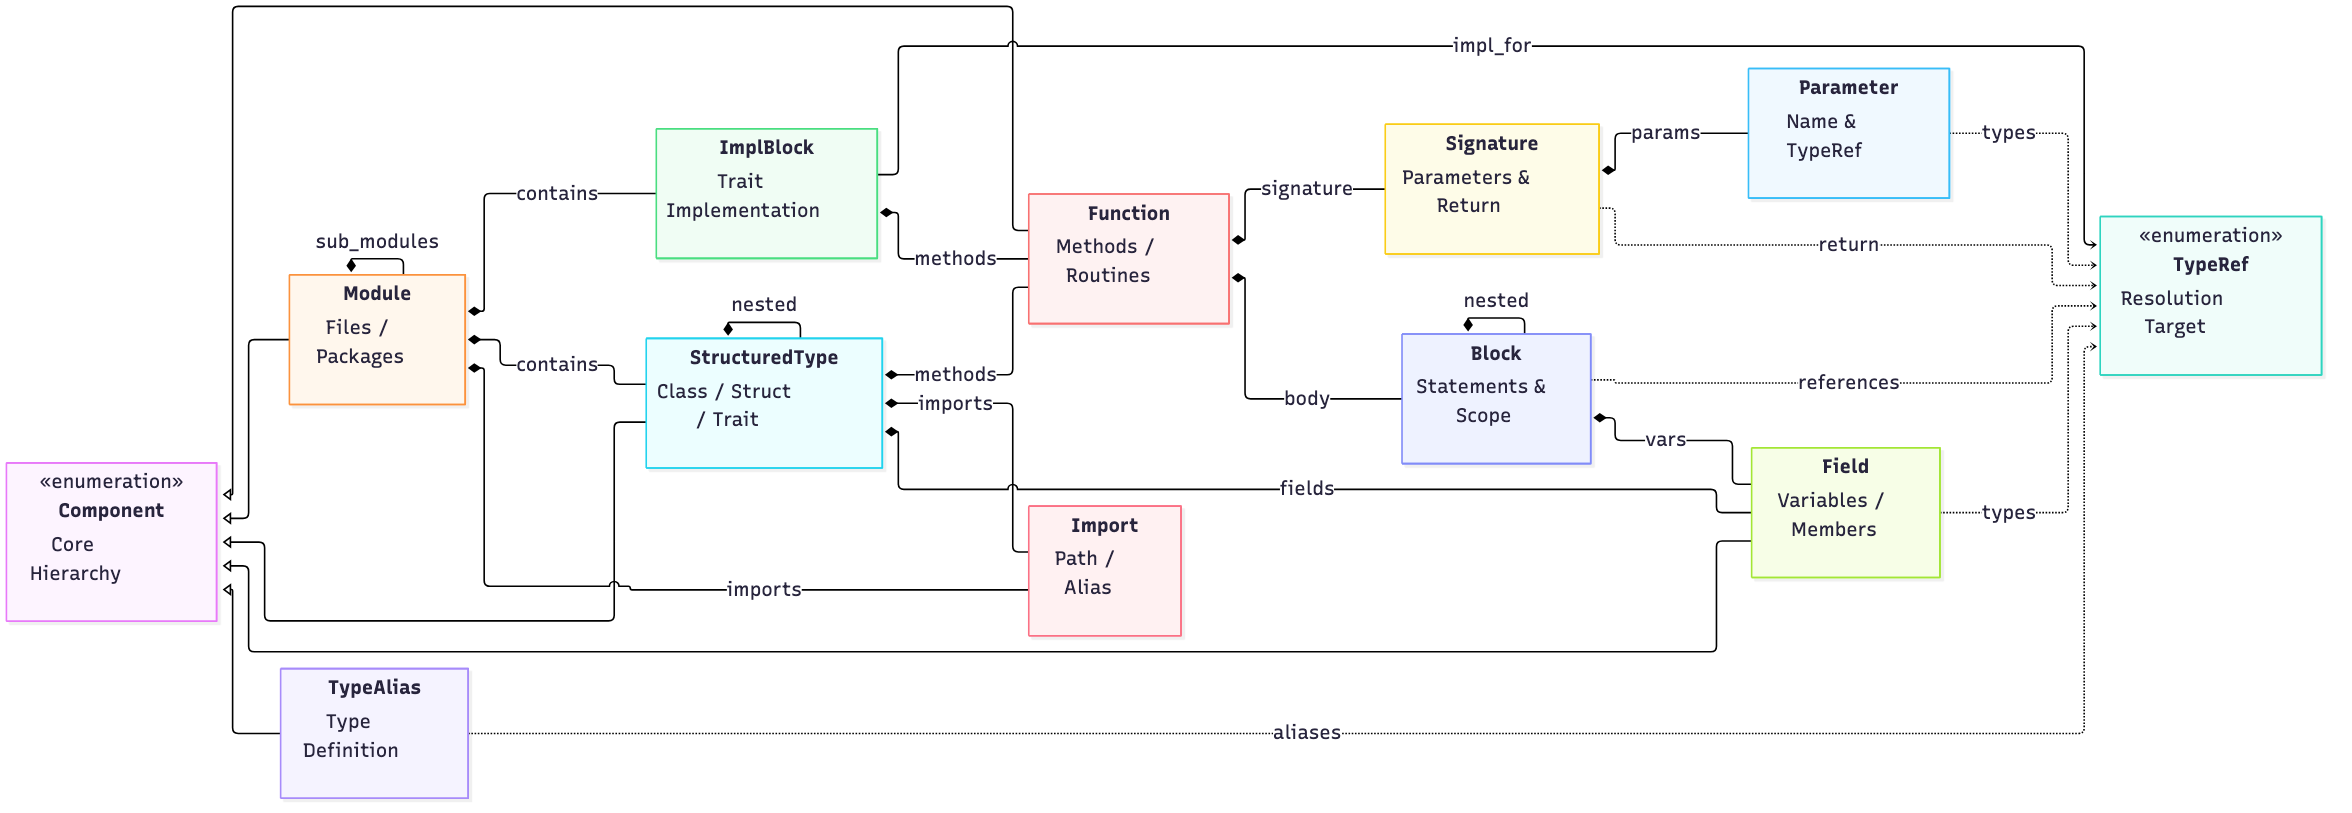
\includegraphics[width=\linewidth,height=0.61\textheight,keepaspectratio]{../images/formal_ir/IR_model_simplified.png}
\end{frame}

% ==============================================================================
% SLIDE 9: FASE 2 - RISOLUZIONE DEI NOMI DISACCOPPIATA
% ==============================================================================
\begin{frame}{Phase 2: Decoupled Name Resolution}{TypeRef Binding and Two-Step Scope Navigation}
  \begin{columns}[c,onlytextwidth]
    \column{0.35\textwidth}
      \cookiekicker{TypeRef Resolution}\par\vspace{0.15em}
      {\footnotesize
      Symbol references (variable types, calls) start as unresolved \texttt{TypeRef}s. Phase 2 binds them to concrete targets.\par}
      \vspace{0.45em}

      \cookiekicker{Two-Step Decoupling}\par\vspace{0.15em}
      {\footnotesize
      \textbf{1. Local Query Building:}\\
      Local symbol stack rewrites references into closed queries, then frees local state.\par\vspace{0.20em}
      \textbf{2. Global Query Execution:}\\
      Evaluates queries deterministically over the global Scope Tree without file-order bias.\par}
      \vspace{0.45em}

      \cookiekicker{Three Query Primitives}\par\vspace{0.20em}
      \cookiebadge{Find} {\scriptsize Lexical climbing}\hspace{0.2em}\\
      \cookiebadge{Extract} {\scriptsize Member descent}\hspace{0.2em}\\
      \cookiebadge{Call} {\scriptsize Return propagation}\par

    \column{0.64\textwidth}
      \centering
      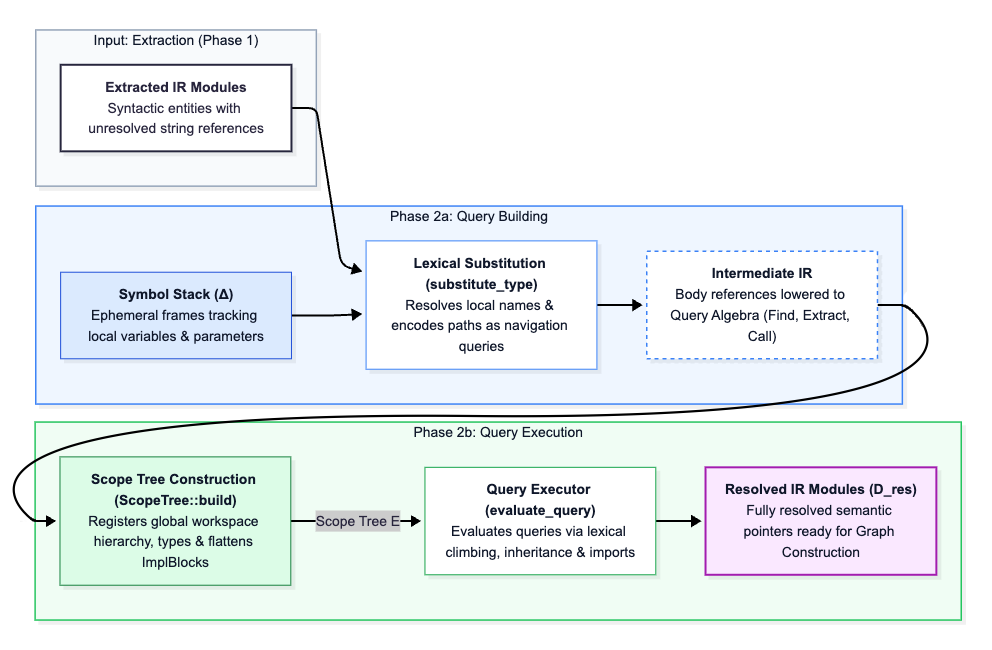
\includegraphics[width=\linewidth,height=0.68\textheight,keepaspectratio]{../images/name_resolution/two_phase_resolution.png}\par\vspace{0.15em}
      {\scriptsize\color{cookieMuted}Two-phase resolution: local stack ($\rho_{\text{build}}$) $\to$ global Scope Tree ($\rho_{\text{exec}}$)\par}
  \end{columns}
\end{frame}



% ==============================================================================
% SLIDE 10: FASE 3 - GRAPH CONSTRUCTION
% ==============================================================================
\begin{frame}{Phase 3: Graph Construction \& Projection}{From Resolved IR Trees to Directed Dependency Multigraphs}
  \begin{columns}[c,onlytextwidth]
    \column{0.56\textwidth}
      \cookiekicker{Construction Pipeline}\par\vspace{0.25em}
      \centering
      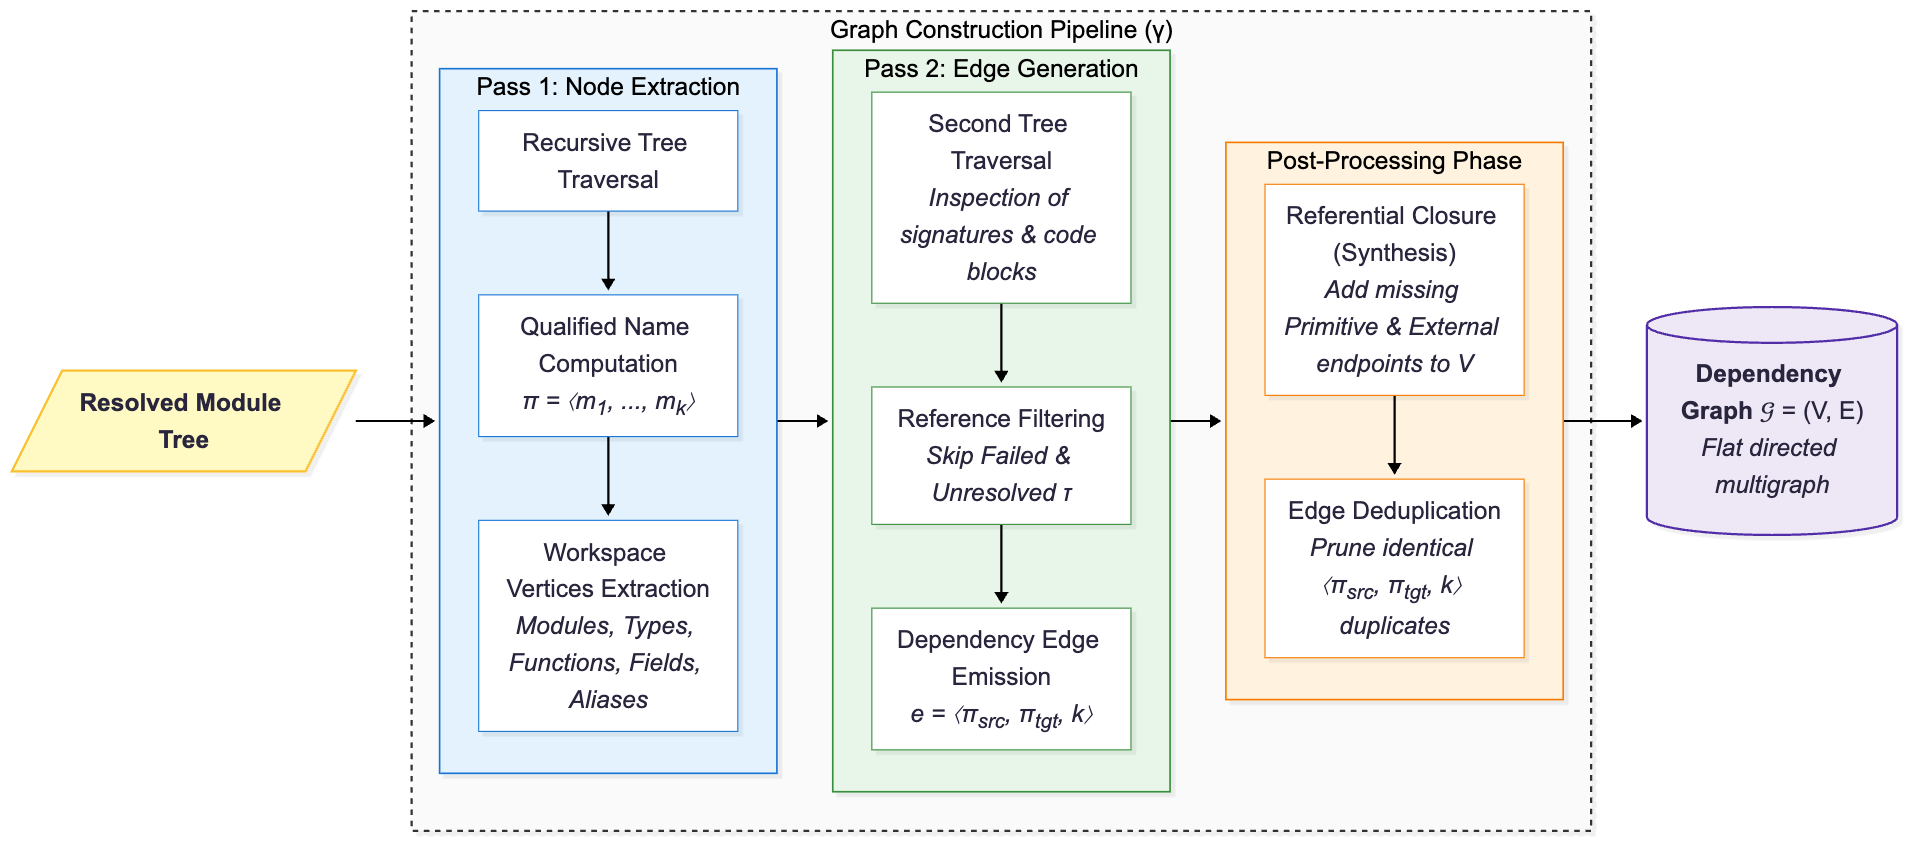
\includegraphics[width=\linewidth,height=0.68\textheight,keepaspectratio]{../images/graph_construction/graph_construction_pipeline.png}\par\vspace{0.2em}
      {\scriptsize\color{cookieMuted}Two-pass traversal: node flattening, edge emission, and referential closure\par}

    \column{0.42\textwidth}
      \cookiekicker{Resulting Dependency Graph}\par\vspace{0.25em}
      \centering
      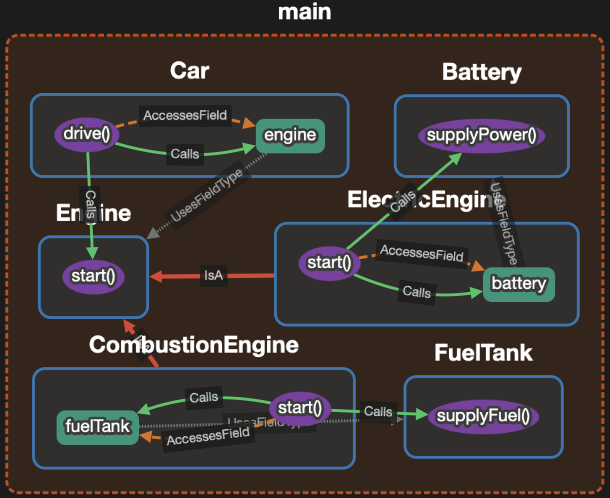
\includegraphics[width=\linewidth,height=0.68\textheight,keepaspectratio]{../images/graph_construction/dep_graph_example.png}\par\vspace{0.2em}
      {\scriptsize\color{cookieMuted}Concrete multigraph: internal components and external endpoints\par}
  \end{columns}
\end{frame}

% ==============================================================================
% SEZIONE 3: VALIDAZIONE SPERIMENTALE
% ==============================================================================
\section{Experimental Validation}

% ==============================================================================
% SLIDE 11: METODOLOGIA SPERIMENTALE & RQ1
% ==============================================================================
\begin{frame}{Experimental Setup}{Research Questions and Background Truth}
  \begin{columns}[T,onlytextwidth]
    \column{0.48\textwidth}
      \cookiekicker{Research Questions}\par\vspace{0.2em}
      {\small
      \textbf{RQ1:} Baseline construct coverage on synthetic oracles\par\vspace{0.25em}
      \textbf{RQ2:} Cross-tool structural alignment (156 repos, 5 languages)\par\vspace{0.25em}
      \textbf{RQ3:} Execution throughput, speedup, and scalability\par}
      \vspace{2.5em}

      \cookiekicker{Baseline Tool Language Coverage}\par\vspace{0.6em}
      {\footnotesize
      \begin{tabular*}{\linewidth}{@{\extracolsep{\fill}}lccccc@{}}
        \toprule
        \textbf{Tool} & \textbf{C} & \textbf{C++} & \textbf{Java} & \textbf{Python} & \textbf{Rust} \\
        \midrule
        \textbf{OmniDeps} & \textcolor{metricGreen}{\tikz[baseline=-0.25ex,line width=0.9pt]{\draw (0,0.07) -- (0.04,0.01) -- (0.12,0.13);}} & \textcolor{metricGreen}{\tikz[baseline=-0.25ex,line width=0.9pt]{\draw (0,0.07) -- (0.04,0.01) -- (0.12,0.13);}} & \textcolor{metricGreen}{\tikz[baseline=-0.25ex,line width=0.9pt]{\draw (0,0.07) -- (0.04,0.01) -- (0.12,0.13);}} & \textcolor{metricGreen}{\tikz[baseline=-0.25ex,line width=0.9pt]{\draw (0,0.07) -- (0.04,0.01) -- (0.12,0.13);}} & \textcolor{metricGreen}{\tikz[baseline=-0.25ex,line width=0.9pt]{\draw (0,0.07) -- (0.04,0.01) -- (0.12,0.13);}} \\
        \textbf{Depends}  & \tikz[baseline=-0.25ex,line width=0.8pt]{\draw (0,0.07) -- (0.04,0.01) -- (0.12,0.13);} & \tikz[baseline=-0.25ex,line width=0.8pt]{\draw (0,0.07) -- (0.04,0.01) -- (0.12,0.13);} & \tikz[baseline=-0.25ex,line width=0.8pt]{\draw (0,0.07) -- (0.04,0.01) -- (0.12,0.13);} & \tikz[baseline=-0.25ex,line width=0.8pt]{\draw (0,0.07) -- (0.04,0.01) -- (0.12,0.13);} & \color{cookieMuted}--- \\
        \textbf{Arcan}    & \tikz[baseline=-0.25ex,line width=0.8pt]{\draw (0,0.07) -- (0.04,0.01) -- (0.12,0.13);} & \tikz[baseline=-0.25ex,line width=0.8pt]{\draw (0,0.07) -- (0.04,0.01) -- (0.12,0.13);} & \tikz[baseline=-0.25ex,line width=0.8pt]{\draw (0,0.07) -- (0.04,0.01) -- (0.12,0.13);} & \tikz[baseline=-0.25ex,line width=0.8pt]{\draw (0,0.07) -- (0.04,0.01) -- (0.12,0.13);} & \color{cookieMuted}--- \\
        \textbf{Entangle} & \color{cookieMuted}--- & \color{cookieMuted}--- & \tikz[baseline=-0.25ex,line width=0.8pt]{\draw (0,0.07) -- (0.04,0.01) -- (0.12,0.13);} & \color{cookieMuted}--- & \tikz[baseline=-0.25ex,line width=0.8pt]{\draw (0,0.07) -- (0.04,0.01) -- (0.12,0.13);} \\
        \bottomrule
      \end{tabular*}}\par

    \column{0.48\textwidth}
      \cookiekicker{RQ1: Synthetic Oracles}\par\vspace{0.15em}
      {\small
      Dedicated benchmark suites with YAML architectural manifests testing constructs in isolation.\par}
      \vspace{0.45em}

      \begin{cookiecard}[title={RQ1 Results:}]
        {\footnotesize Successfully validated against all five language benchmarks, showing the baseline soundness of the approach.\par}
      \end{cookiecard}
      \vspace{0.7em}

      \cookiekicker{Scope Limitation}\par\vspace{0.15em}
      \begin{itemize}
        \footnotesize
        \item Verifies query correctness in a controlled setting.\par\vspace{0.15em}
        \item \textbf{Does not guarantee generalization} to real-world codebases.\par\vspace{0.15em}
        \item Motivates comparative evaluation against established analyzers.\par
      \end{itemize}
  \end{columns}
\end{frame}

% ==============================================================================
% SLIDE 12: METODOLOGIA CROSS-TOOL & COMPLETAMENTO
% ==============================================================================
\begin{frame}{Cross-Tool Methodology \& Feasibility}{Graph Harmonization, Similarity Metrics, and Analysis Completion}
  \begin{columns}[T,onlytextwidth]
    \column{0.48\textwidth}
      \cookiekicker{Metamodel Heterogeneity}\par\vspace{0.15em}
      \small
      Direct intersection fails due to representation disparities across tools:\par
      \begin{itemize}
        \item \textbf{Granularity:} Members (methods) vs. types (classes)\par
        \item \textbf{Taxonomy:} Divergent relation vocabularies\par
        \item \textbf{Naming:} File paths vs. fully qualified identifiers\par
      \end{itemize}
      \vspace{0.45em}

      \cookiekicker{Graph Harmonization (Graph-Synchron)}\par\vspace{0.15em}
      \small
      Automated normalization pipeline:\par
      \begin{itemize}
        \item \textbf{Path Normalization} \& canonical package synthesis\par\vspace{0.15em}
        \item \textbf{Member Lifting} to enclosing type\par\vspace{0.15em}
        \item \textbf{Taxonomy Alignment} \par
      \end{itemize}
      \vspace{0.45em}

     

    \column{0.48\textwidth}
      \cookiekicker{Execution Completion on 156 Repositories}\par\vspace{0.15em}
      {\scriptsize
      \begin{tabular*}{\linewidth}{@{\extracolsep{\fill}}lcccc@{}}
        \toprule
        \textbf{Language} & \textbf{OmniDeps} & \textbf{Depends} & \textbf{Arcan} & \textbf{Entangle} \\
        \midrule
        \textbf{C} (31)      & \textbf{31} (100\%) & 30 (97\%)  & 27 (87\%)  & \color{cookieMuted}--- \\
        \textbf{C++} (31)    & \textbf{30} (97\%)  & 25 (81\%)  & 16 (52\%)  & \color{cookieMuted}--- \\
        \textbf{Java} (32)   & \textbf{32} (100\%) & 31 (97\%)  & 18 (56\%)  & 19 (59\%) \\
        \textbf{Python} (30) & \textbf{30} (100\%) & 29 (97\%)  & 0 (0\%)    & \color{cookieMuted}--- \\
        \textbf{Rust} (32)   & \textbf{32} (100\%) & \color{cookieMuted}--- & \color{cookieMuted}--- & 0 (0\%) \\
        \midrule
        \textbf{Total} (156) & \textbf{155 (99.4\%)} & 115 (93\%) & 61 (49\%)  & 19 (30\%) \\
        \bottomrule
      \end{tabular*}}\par
      \vspace{0.35em}
       \cookiekicker{Graph Comparison Metrics}\par\vspace{0.05em}
      {\scriptsize\setlength{\abovedisplayskip}{1pt}\setlength{\belowdisplayskip}{1pt}\setlength{\jot}{1.5pt}
      \begin{align*}
        J(A, B) &= \frac{|A \cap B| + 1}{|A \cup B| + 1} && \text{\footnotesize (Smoothed Jaccard)} \\
        \text{Inf}(A, B) &= \frac{|B \setminus A|}{|A \cap B|}, \quad \text{Sup} = \frac{|A \setminus B|}{|A \cap B|} && \text{\footnotesize (Omission / Novelty)} \\
        \Delta_{B \setminus A} &= \frac{|E_B \setminus E_A|}{|E_B|}, \quad \Delta_{A \setminus B} = \frac{|E_A \setminus E_B|}{|E_A|} && \text{\footnotesize (Per-Category Rate)}
      \end{align*}}\par
  \end{columns}
\end{frame}

% ==============================================================================
% SLIDE 13: RISULTATI RQ2 - ALLINEAMENTO STRUTTURALE
% ==============================================================================
\begin{frame}{RQ2: Cross-Tool Structural Alignment}{Object-Oriented Parity, Dynamic Entity Lifting, and First Rust Baseline}
  \begin{columns}[T,onlytextwidth]
    \column{0.50\textwidth}
      \cookiekicker{Cross-Tool Agreement Across Paradigms}\par\vspace{0.15em}
      {\scriptsize
      \begin{tabular*}{\linewidth}{@{\extracolsep{\fill}}lccccc@{}}
        \toprule
        \textbf{Lang} & \textbf{Baseline} & $\mathbf{J_{\text{nodes}}}$ & \textbf{Omission} & \textbf{Novelty} & $\mathbf{J_{\text{edges}}}$ \\
        \midrule
        \textbf{Java}   & Depends  & \textbf{0.814} & \textbf{2.1\%} & 28.6\% & 0.587 \\
                        & Entangle & \textbf{0.770} & 19.6\%         & 19.9\% & 0.600 \\
                        & Arcan    & 0.630          & \textbf{0.3\%} & 79.6\% & 0.580 \\
        \midrule
        \textbf{Python} & Depends  & \textbf{0.852} & \textbf{4.8\%} & 16.1\% & 0.368$^*$ \\
        \midrule
        \textbf{C / C++}& \multicolumn{5}{c}{\textit{Detailed on next slide (preprocessor dynamics)}} \\
        \bottomrule
      \end{tabular*}}\par
      \vspace{0.15em}
      {\tiny\color{cookieMuted}$^*$Behavioral edges only (excludes syntactic imports omitted by baseline).\par}
      \vspace{0.25em}

      \cookiekicker{Empirical Takeaways}\par\vspace{0.15em}
      {\scriptsize
      \begin{itemize}\setlength{\itemsep}{0.20em}
        \item \textbf{Object-Oriented Parity (Java):} Near-identical topology with mature compiler tools; misses $\le 2.1\%$ of nodes without JVM/bytecode.
        \item \textbf{Dynamic Typing \& Lifting (Python):} Harmonizing method-local test fixtures raises node Jaccard to \textbf{0.852} (omission $33.2\% \to 4.8\%$).
        \item \textbf{Polyglot Workspace Traversal:} Extracts across all languages (e.g. Rust core in Pydantic), unlike single-language baselines.
      \end{itemize}\par}
      \vspace{0.25em}
      \cookiebadge{Java $J_{\text{nodes}} > 0.81$} \hspace{0.2em}
      \cookiebadge{Python $\text{Inf}=4.8\%$} \hspace{0.2em}
      \cookiebadge{Rust 100\%}

    \column{0.48\textwidth}
      \cookiekicker{Pairwise Similarity in Java}\par\vspace{0.2em}
      \centering
      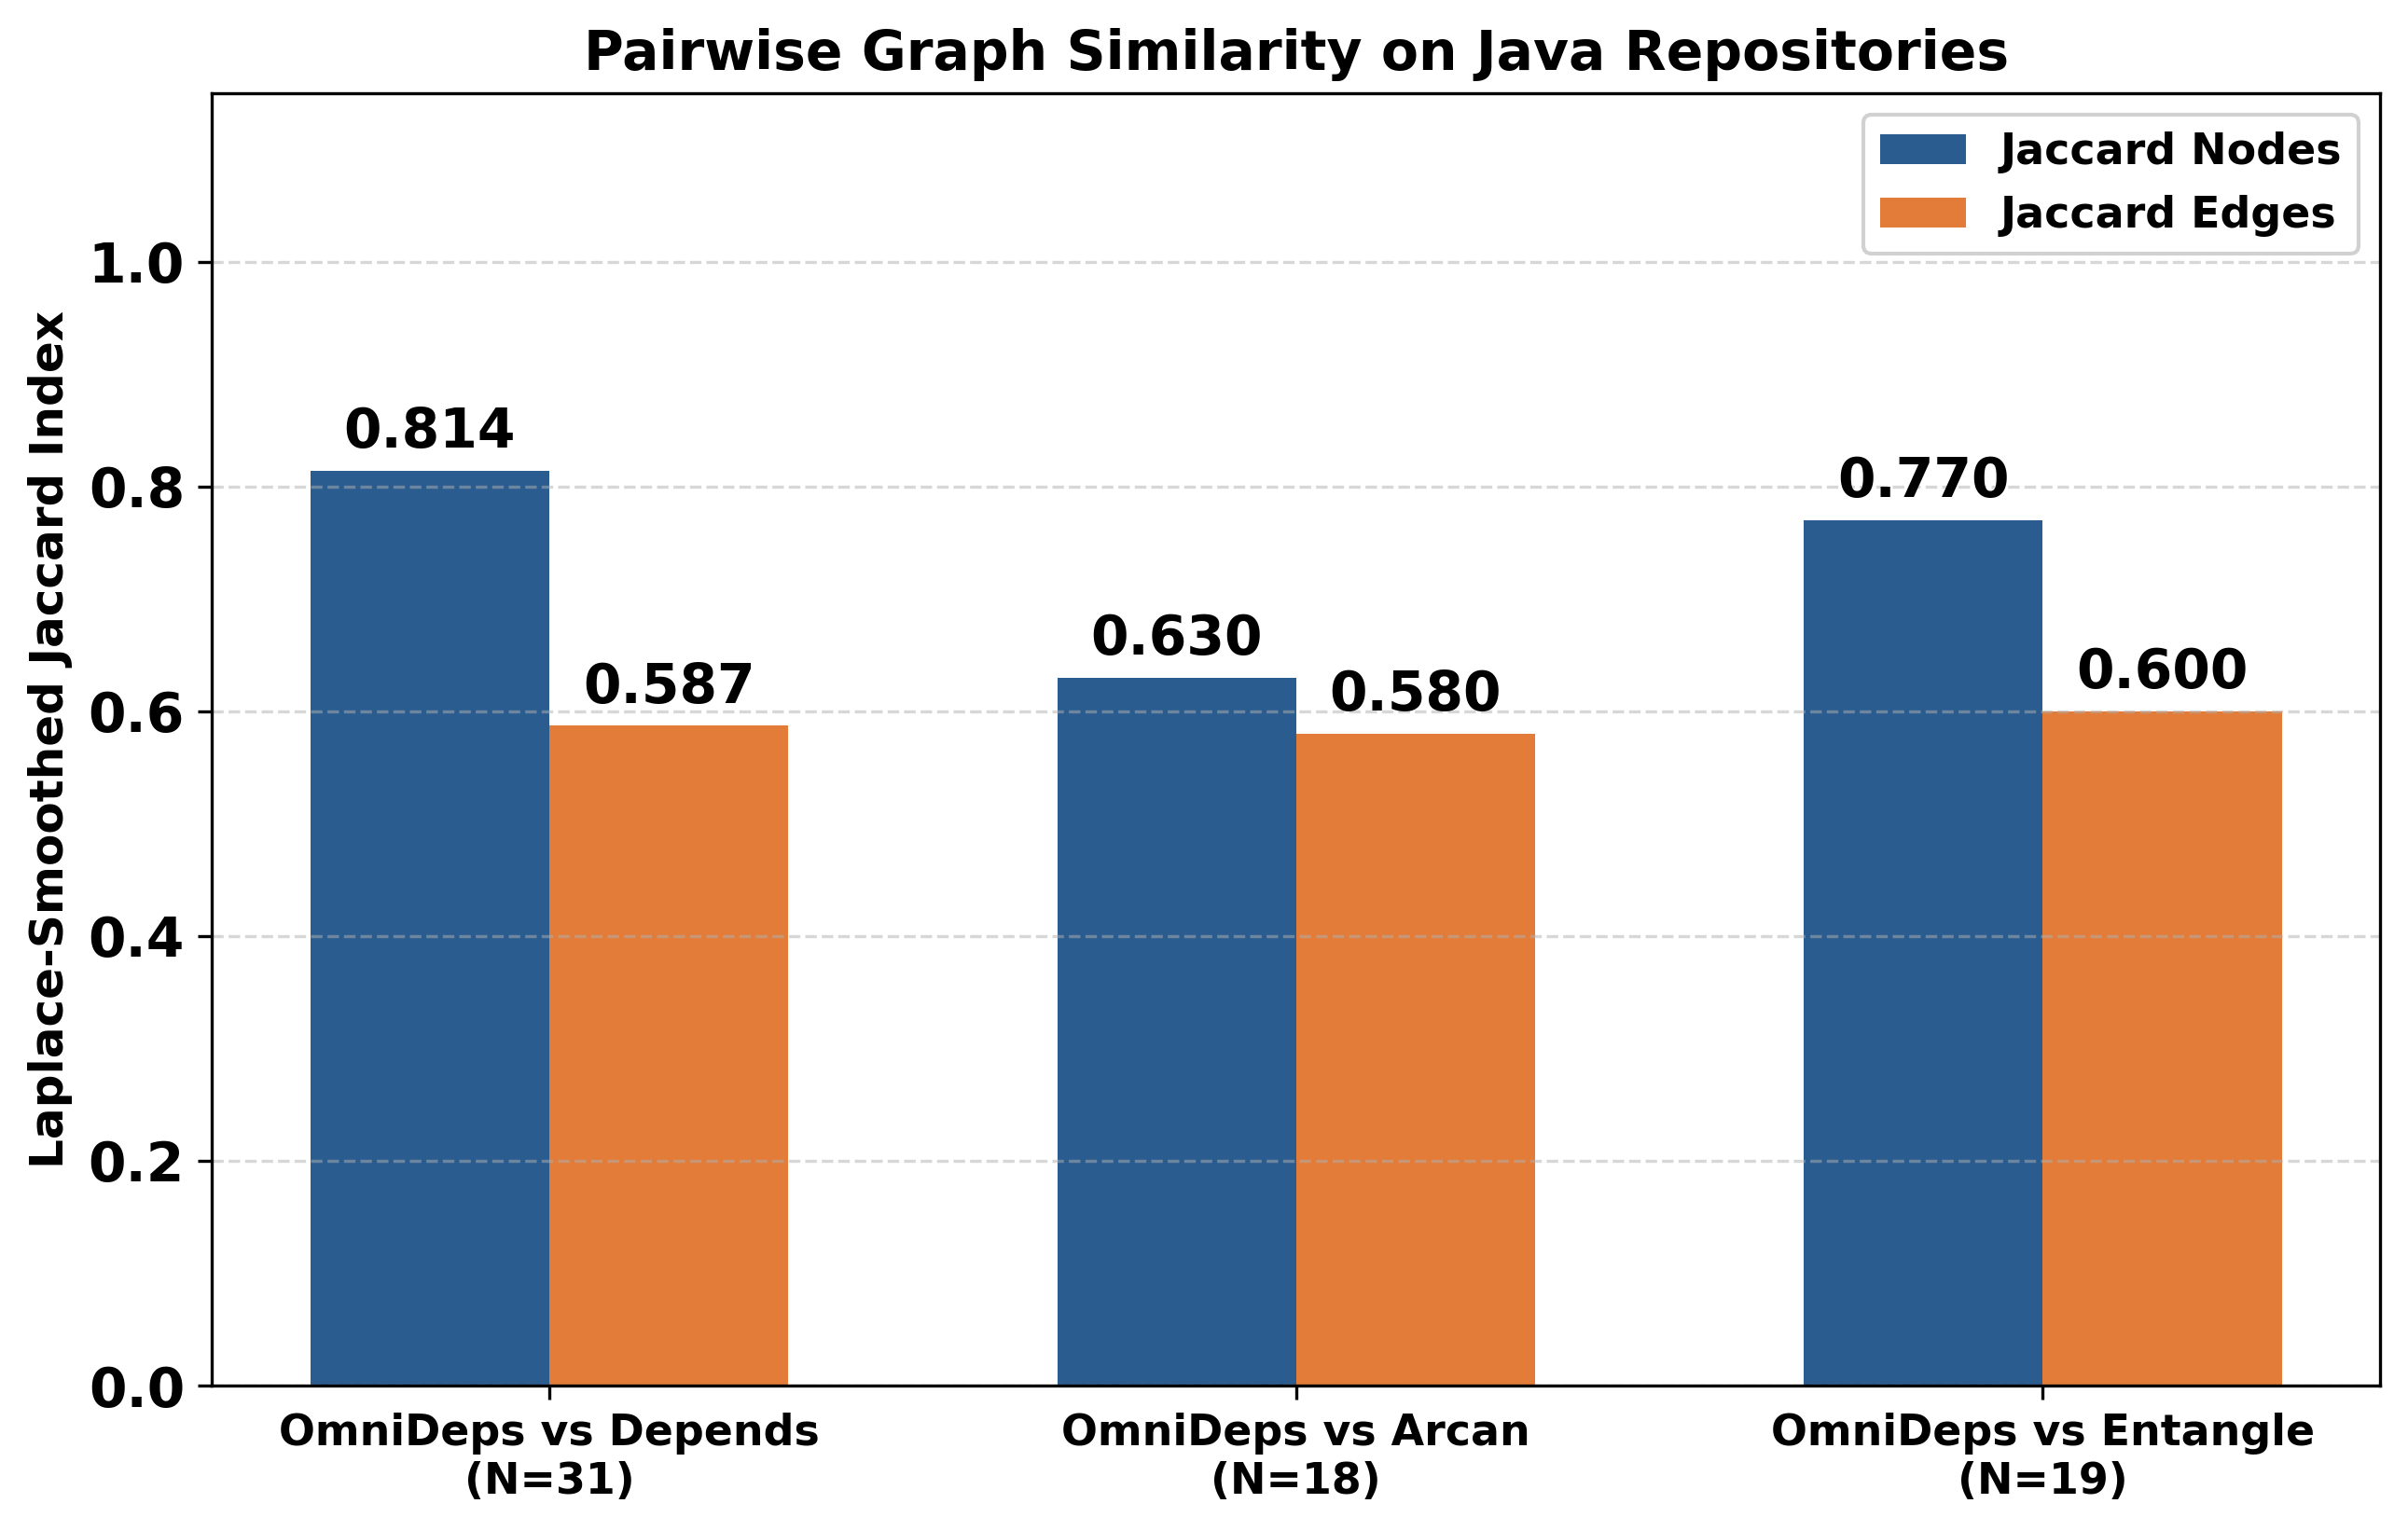
\includegraphics[width=\linewidth,height=0.60\textheight,keepaspectratio]{../images/evaluation/comparisons/summary-jaccard-java.png}\par\vspace{0.2em}
      {\scriptsize\color{cookieMuted}Smoothed Jaccard indices across Java projects against Depends, Arcan and Entangle\par}
  \end{columns}
\end{frame}

% ==============================================================================
% SLIDE 14: RISULTATI RQ2 - DEEP DIVE C & C++
% ==============================================================================
\begin{frame}{RQ2: Structural Alignment in C \& C++}{The Preprocessor Dilemma and Ontological Disparity}
  \begin{columns}[T,onlytextwidth]
    \column{0.48\textwidth}
      \cookiekicker{Cross-Tool Agreement in C \& C++}\par\vspace{0.15em}
      {\scriptsize
      \begin{tabular*}{\linewidth}{@{\extracolsep{\fill}}llccc@{}}
        \toprule
        \textbf{Lang} & \textbf{Baseline / Mode} & $\mathbf{J_{\text{nodes}}}$ & $\mathbf{J_{\text{edges}}}$ & \textbf{Outcome} \\
        \midrule
        \textbf{C}   & Depends (Raw)       & 0.191 & 0.115 & Baseline \\
                     & Depends (Preproc.)  & \textbf{0.204} & \textbf{0.136} & +18\% Edges \\
        \midrule
        \textbf{C++} & Depends (Raw)       & 0.143 & 0.081 & Baseline \\
                     & Depends (Preproc.)  & \textbf{0.192} & \textbf{0.165} & \textbf{2$\times$ Recall} \\
        \midrule
        \textbf{C/C++}& Arcan (File-level) & $\le 0.01$ & $\le 0.00$ & Ontological \\
        \midrule
        \textbf{C} (\texttt{sds}) & Depends & \textbf{1.000} & \textbf{1.000} & Perfect Parity \\
        \bottomrule
      \end{tabular*}}\par
      \vspace{0.35em}

      \cookiekicker{Key Empirical Findings}\par\vspace{0.15em}
      {\scriptsize
      \begin{itemize}\setlength{\itemsep}{0.20em}
        \item \textbf{Preprocessor Dilemma:} Macro expansion doubles C++ edge recall ($0.081 \to 0.165$), but header inlining duplicates types across translation units.
        \item \textbf{Ontological Disparity (Arcan):} Arcan tracks physical files/headers for smell detection; OmniDeps extracts logical AST types ($V_A \cap V_B = \emptyset$).
        \item \textbf{Isolated Modular Soundness:} On clean modular libraries like \texttt{antirez/sds}, extraction achieves \textbf{perfect agreement ($J = 1.0$)}.
      \end{itemize}\par}
      \vspace{0.25em}
      \cookiebadge{Preproc: $2\times$ Edges} \hspace{0.2em}
      \cookiebadge{\texttt{sds} $J=1.0$} \hspace{0.2em}
      \cookiebadge{Ontological Disparity}

    \column{0.48\textwidth}
      \cookiekicker{Impact of Macro Preprocessing}\par\vspace{0.2em}
      \centering
      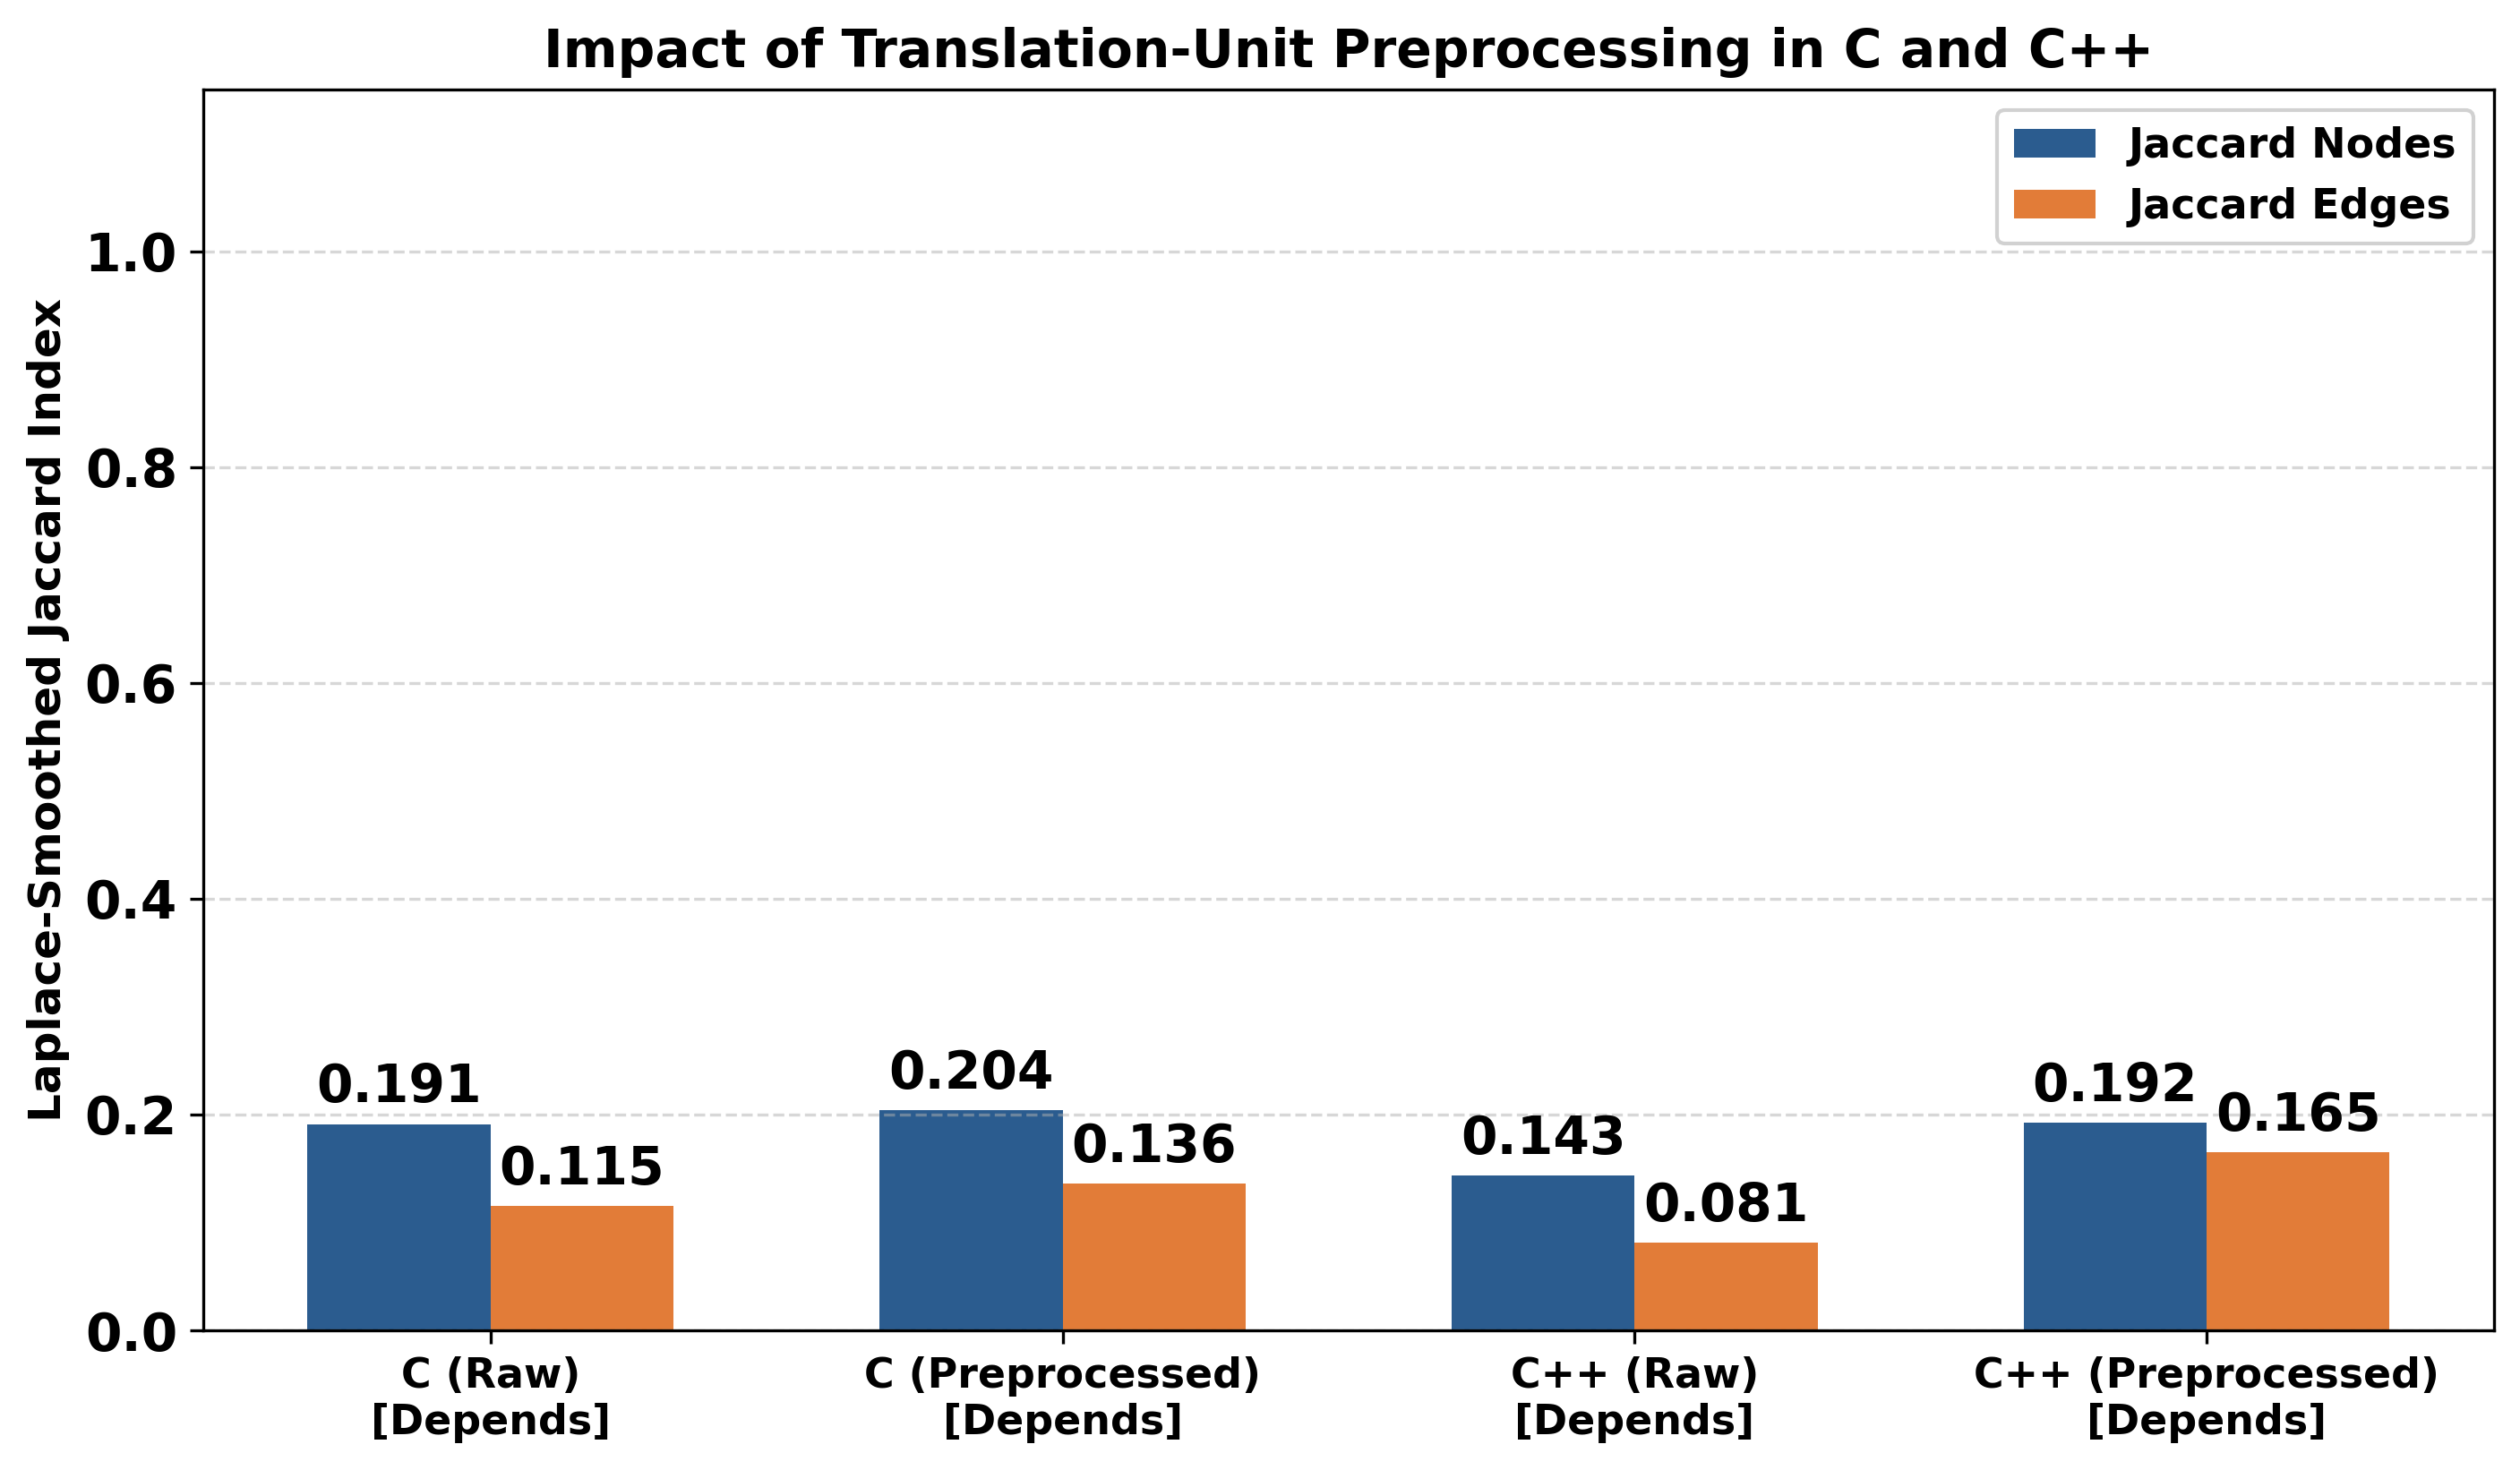
\includegraphics[width=\linewidth,height=0.48\textheight,keepaspectratio]{../images/evaluation/comparisons/summary-jaccard-c-cpp-preprocessing.png}\par\vspace{0.2em}
      {\scriptsize\color{cookieMuted}Jaccard similarity before and after macro expansion (\texttt{clang -E}) against Depends across 31 C and 22 C++ repositories\par}
  \end{columns}
\end{frame}

% ==============================================================================
% SLIDE 15: RISULTATI RQ3 - PRESTAZIONI & SCALABILITÀ
% ==============================================================================
\begin{frame}{RQ3: Runtime Performance and Scalability}{Linear Scaling and Throughput for Continuous Auditing}
  \begin{columns}[T,onlytextwidth]
    \column{0.42\textwidth}
      \cookiekicker{Computational Efficiency}\par\vspace{0.2em}
      {\small
      \begin{itemize}\setlength{\itemsep}{0.35em}
        \item \textbf{Strict $O(N)$ Linear Scaling:} Single-pass parsing and scoped resolution scale proportionally with LOC.
        \item \textbf{Seconds on 1M+ LOC:} Extraction finishes in seconds even on large codebases, with flat memory usage.
        \item \textbf{High Throughput:} Sustained mean of \textbf{\textcolor{metricGreen}{74k+ LOC/s}}, consistently matching or exceeding baselines.
        \item \textbf{Continuous CI/CD:} Fast runtimes enable practical adoption in automated quality gates.
      \end{itemize}\par}
      \vspace{0.4em}
      \cookiebadge{$O(N)$ Linear} \hspace{0.2em}
      \cookiebadge{Seconds on 1M+ LOC}

    \column{0.56\textwidth}
      \cookiekicker{Execution Time vs. Codebase Size}\par\vspace{0.15em}
      \centering
      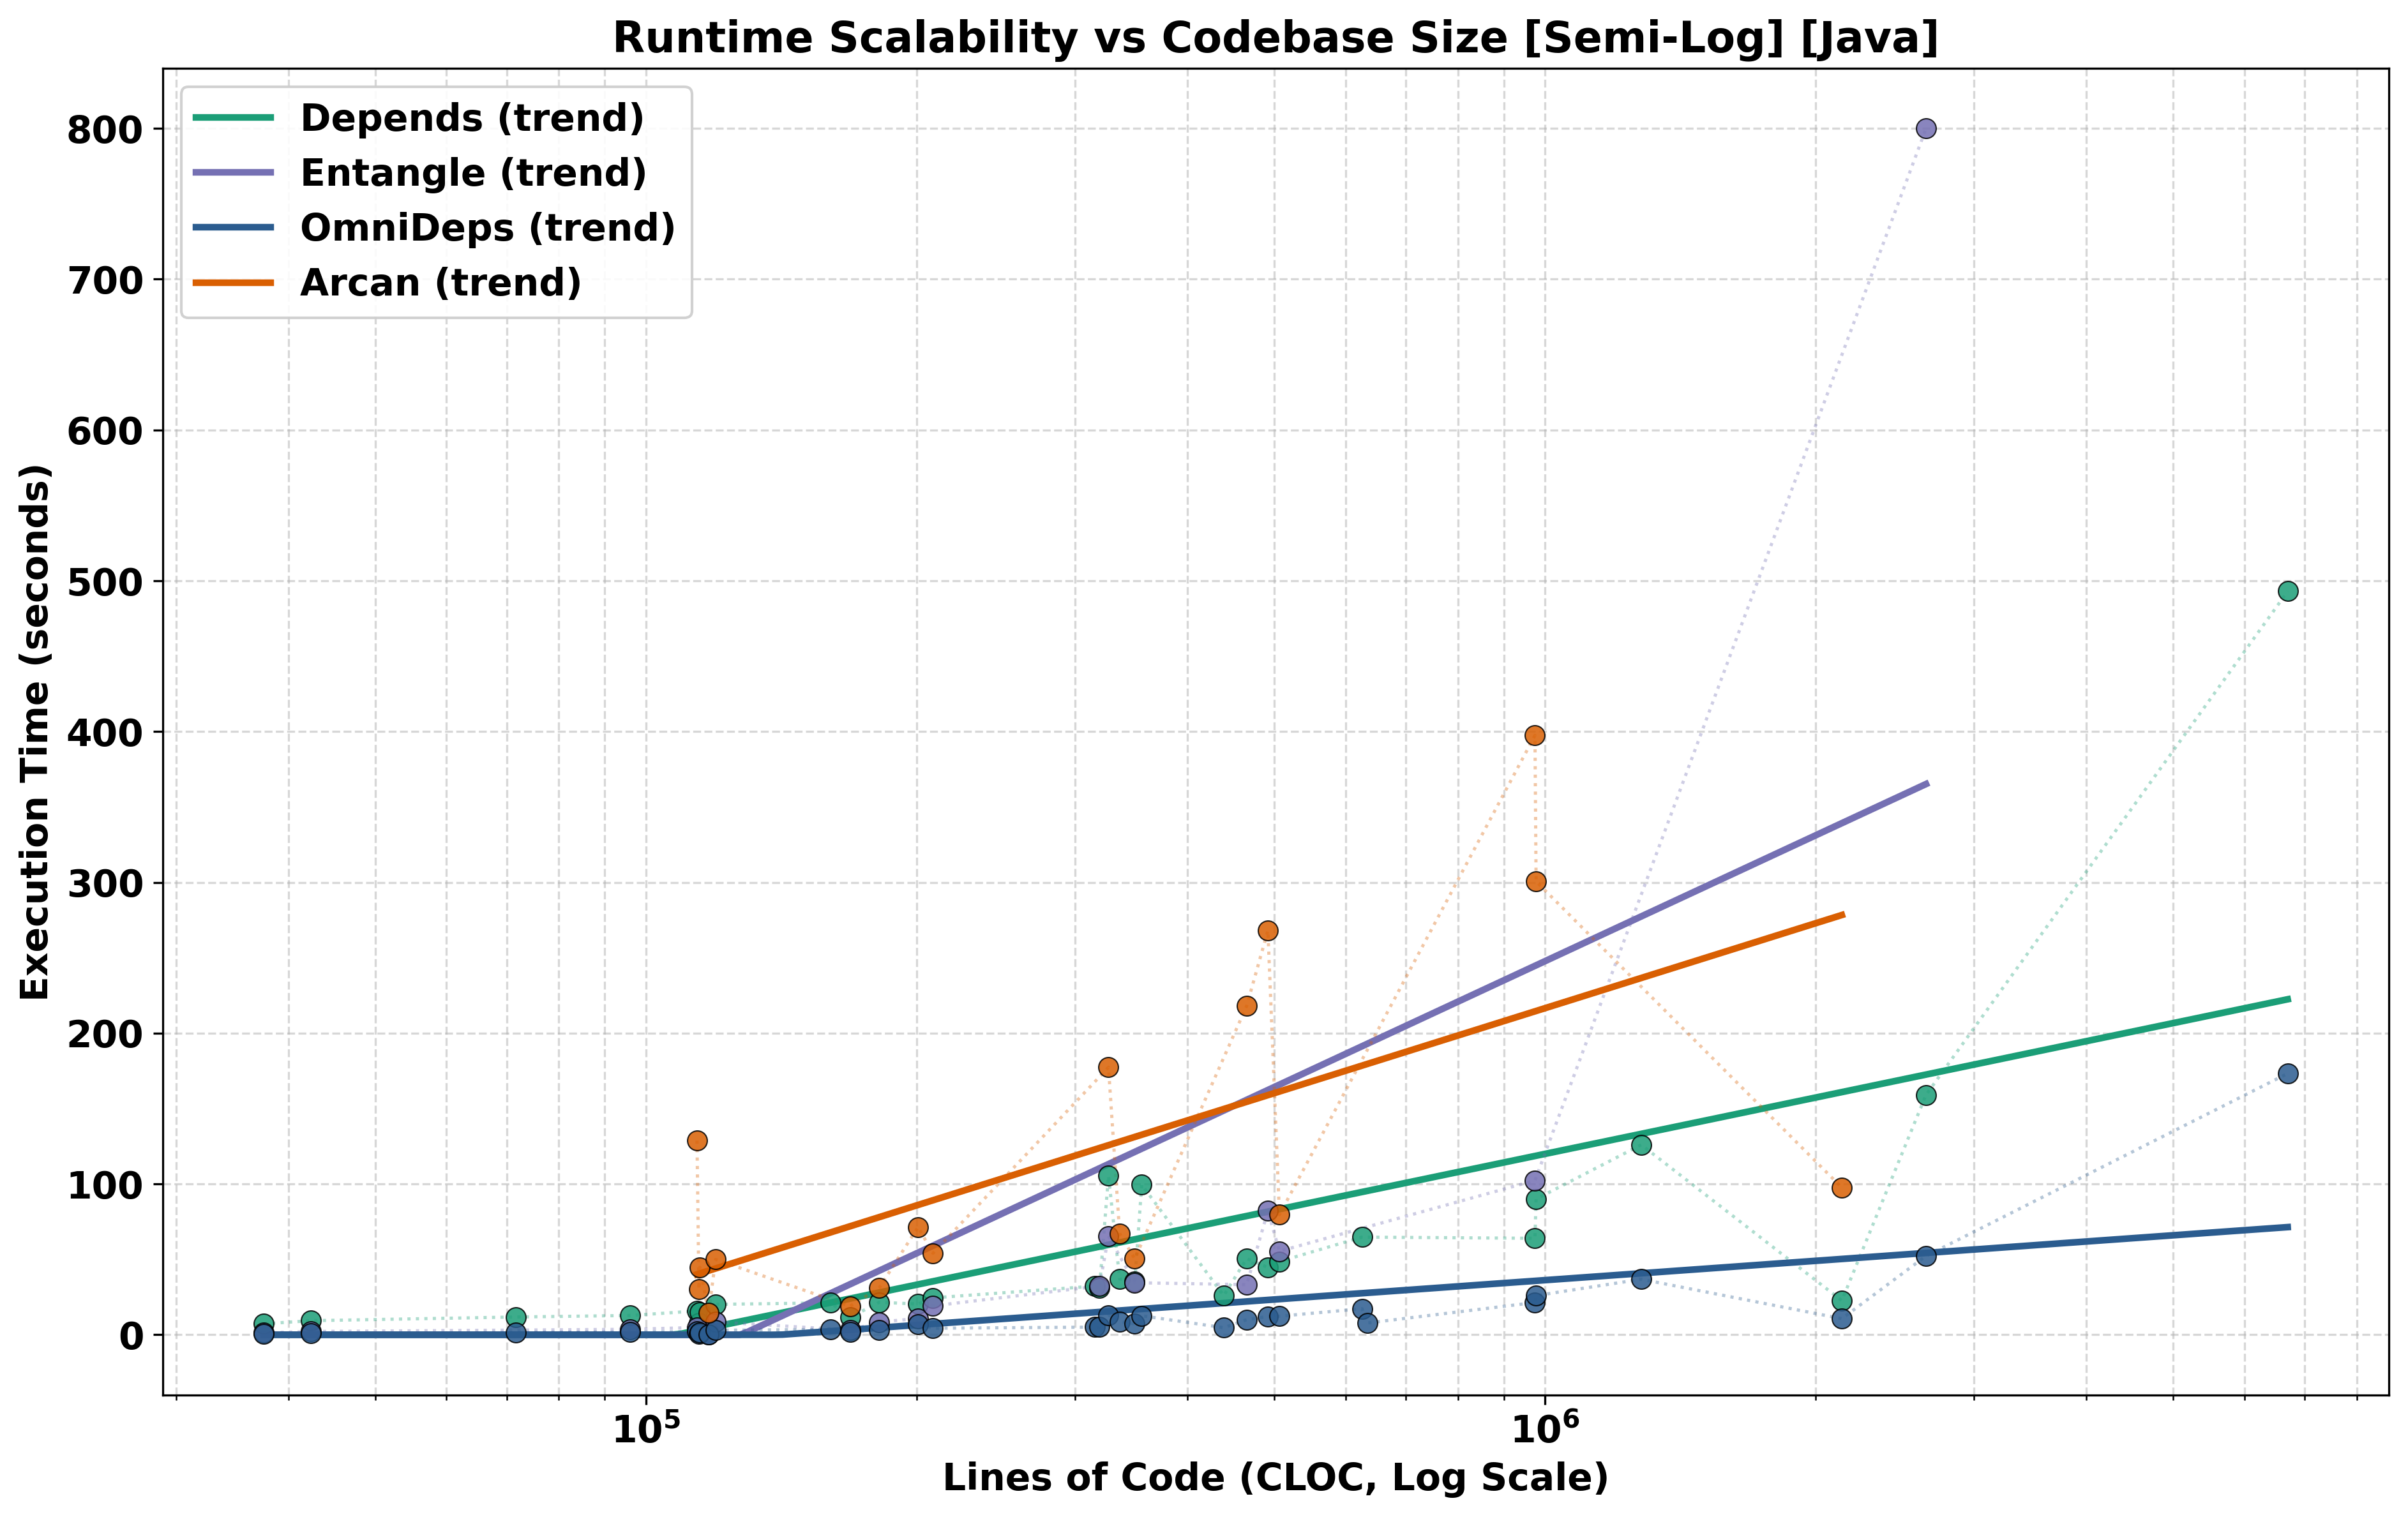
\includegraphics[width=\linewidth,height=0.62\textheight,keepaspectratio]{../images/evaluation/times/graph-cloc-log-java.png}\par\vspace{0.15em}
      {\scriptsize\color{cookieMuted}Wall-clock extraction time vs. codebase size (LOC) across Java repositories on semi-log scale\par}
  \end{columns}
\end{frame}

% ==============================================================================
% SLIDE 16: CONCLUSIONI E SVILUPPI FUTURI
% ==============================================================================
\begin{frame}{Conclusions \& Outlook}{Viability of Language-Agnostic Extraction and Future Research Directions}
    Language-agnostic, syntax-directed extraction proves to be a \textbf{viable and sound approach} for architectural
    dependency analysis: it recovers reliable dependency graphs in seconds without compiler or build-system friction,
     while establishing clear methodological boundaries and open research avenues.\par
  \vspace{1em}

  \begin{columns}[T,onlytextwidth]
    \column{0.49\textwidth}
      \cookiekicker{Threats to Validity}\par\vspace{0.15em}
      {\footnotesize
      \begin{itemize}\setlength{\itemsep}{0.25em}
        \item \textbf{Absence of Real-World Oracles:} Evaluating against mature analyzers measures cross-tool concordance rather than absolute correctness.
        \item \textbf{Harmonization Abstraction:} Semantic entity lifting evaluates macro-architectural (type-level) convergence, abstracting statement details.
        \item \textbf{Syntactic Premise in C/C++:} Macro masking challenges raw CST fidelity, forcing a trade-off with header duplication.
      \end{itemize}\par}

    \column{0.49\textwidth}
      \cookiekicker{Future Research Directions}\par\vspace{0.15em}
      {\footnotesize
      \begin{itemize}\setlength{\itemsep}{0.25em}
        \item \textbf{Link-Time Symbol Deduplication:} Linker-like reconciliation pass to merge duplicated C/C++ header declarations across compilation units.
        \item \textbf{Non-Imperative Paradigms:} Generalizing query algebra to functional composition (Haskell/OCaml) and declarative logic relations.
        \item \textbf{Cross-Language Boundaries:} Tracing foreign function interfaces (FFI/JNI) across language boundaries via the shared Scope Tree.
      \end{itemize}\par}
  \end{columns}
  \vspace{0.35em}
\end{frame}

% ==============================================================================
% SLIDE 17: CHIUSURA & Q&A
% Slide personalizzata con sfondo Unimib Blue, QR code Zenodo e niente mascotte
% ==============================================================================
\begin{frame}[plain,noframenumbering]
  
\begin{tikzpicture}[remember picture,overlay]
    \fill[unimibBlue] (current page.south west) rectangle (current page.north east);
    % Cerchi decorativi
    \draw[white,opacity=0.08,line width=3pt] ($(current page.north east)+(-0.15\paperwidth,-0.15\paperheight)$) circle[radius=0.18\paperheight];
    \draw[white,opacity=0.05,line width=2pt] ($(current page.south west)+(0.20\paperwidth,0.20\paperheight)$) circle[radius=0.12\paperheight];
  \end{tikzpicture}%
  \vspace*{0.02\paperheight}%
  \begin{columns}[c,onlytextwidth]
    \column{0.58\textwidth}
      {\scriptsize\color{white!70} UNIVERSITÀ DEGLI STUDI DI MILANO-BICOCCA \quad $\cdot$ \quad DISCo}\par\vspace{0.35em}
      {\fontsize{22}{26}\selectfont\bfseries\color{white} Thanks for your\\ attention!}\par\vspace{0.55em}
      {\small\color{white!95}\textbf{A Language-Agnostic Framework\\ for Dependency Extraction}}\par\vspace{0.55em}
      {\color{white!35}\rule{0.28\paperwidth}{0.8pt}}\par\vspace{0.75em}
      \begin{columns}[t,onlytextwidth]
        \column{0.48\textwidth}
          {\scriptsize\color{white!70} CANDIDATE\par}\vspace{0.15em}
          {\normalsize\bfseries\color{white} Christian Ferrario\par}\vspace{0.1em}
          {\scriptsize\color{white!70}\texttt{c.ferrario30@campus.unimib.it}\par}
        \column{0.52\textwidth}
          {\scriptsize\color{white!70} SUPERVISORS\par}\vspace{0.15em}
          {\normalsize\bfseries\color{white} Prof.~Francesca Arcelli Fontana\par}
          {\scriptsize\color{white!80} Supervisor\par}\vspace{0.25em}
          {\normalsize\bfseries\color{white} Dr.~Francesco Refolli\par}
          {\scriptsize\color{white!80} Co-Supervisor\par}
      \end{columns}
      \vspace{0.9em}
      {\small\itshape\color{white!85} Questions and discussion are welcome\par}

    \column{0.38\textwidth}
      \centering
      \begin{tcolorbox}[
        colback=white,
        colframe=white,
        arc=3.5mm,
        boxrule=0pt,
        width=0.92\linewidth,
        halign=center,
        valign=center,
        top=4.5mm,bottom=4.5mm,left=3mm,right=3mm
      ]
        \href{https://doi.org/10.5281/zenodo.23315197}{\color{black}\qrcode[height=2.35cm]{https://doi.org/10.5281/zenodo.23315197}}\par
        \vspace{0.45em}
        {\small\bfseries\color{unimibBlue} Replicability Package}\par\vspace{0.15em}
        {\scriptsize\color{cookieMuted} Zenodo DOI: 10.5281/zenodo.23315197\par}\vspace{0.25em}
        {\tiny\texttt{\color{cookieDemoBlue}github.com/FerrarioChristian/omnideps}\par}
      \end{tcolorbox}
  \end{columns}
\end{frame}

% ==============================================================================
% APPENDIX / BACKUP SLIDES
% ==============================================================================
\appendix

% BACKUP SLIDE 1: Cross-Language Pairwise Similarity Overview
\begin{frame}[noframenumbering]{Appendix: Cross-Language Graph Similarity}{Pairwise Laplace-Smoothed Jaccard Index Across All Analyzed Tool Pairs}
  \centering
  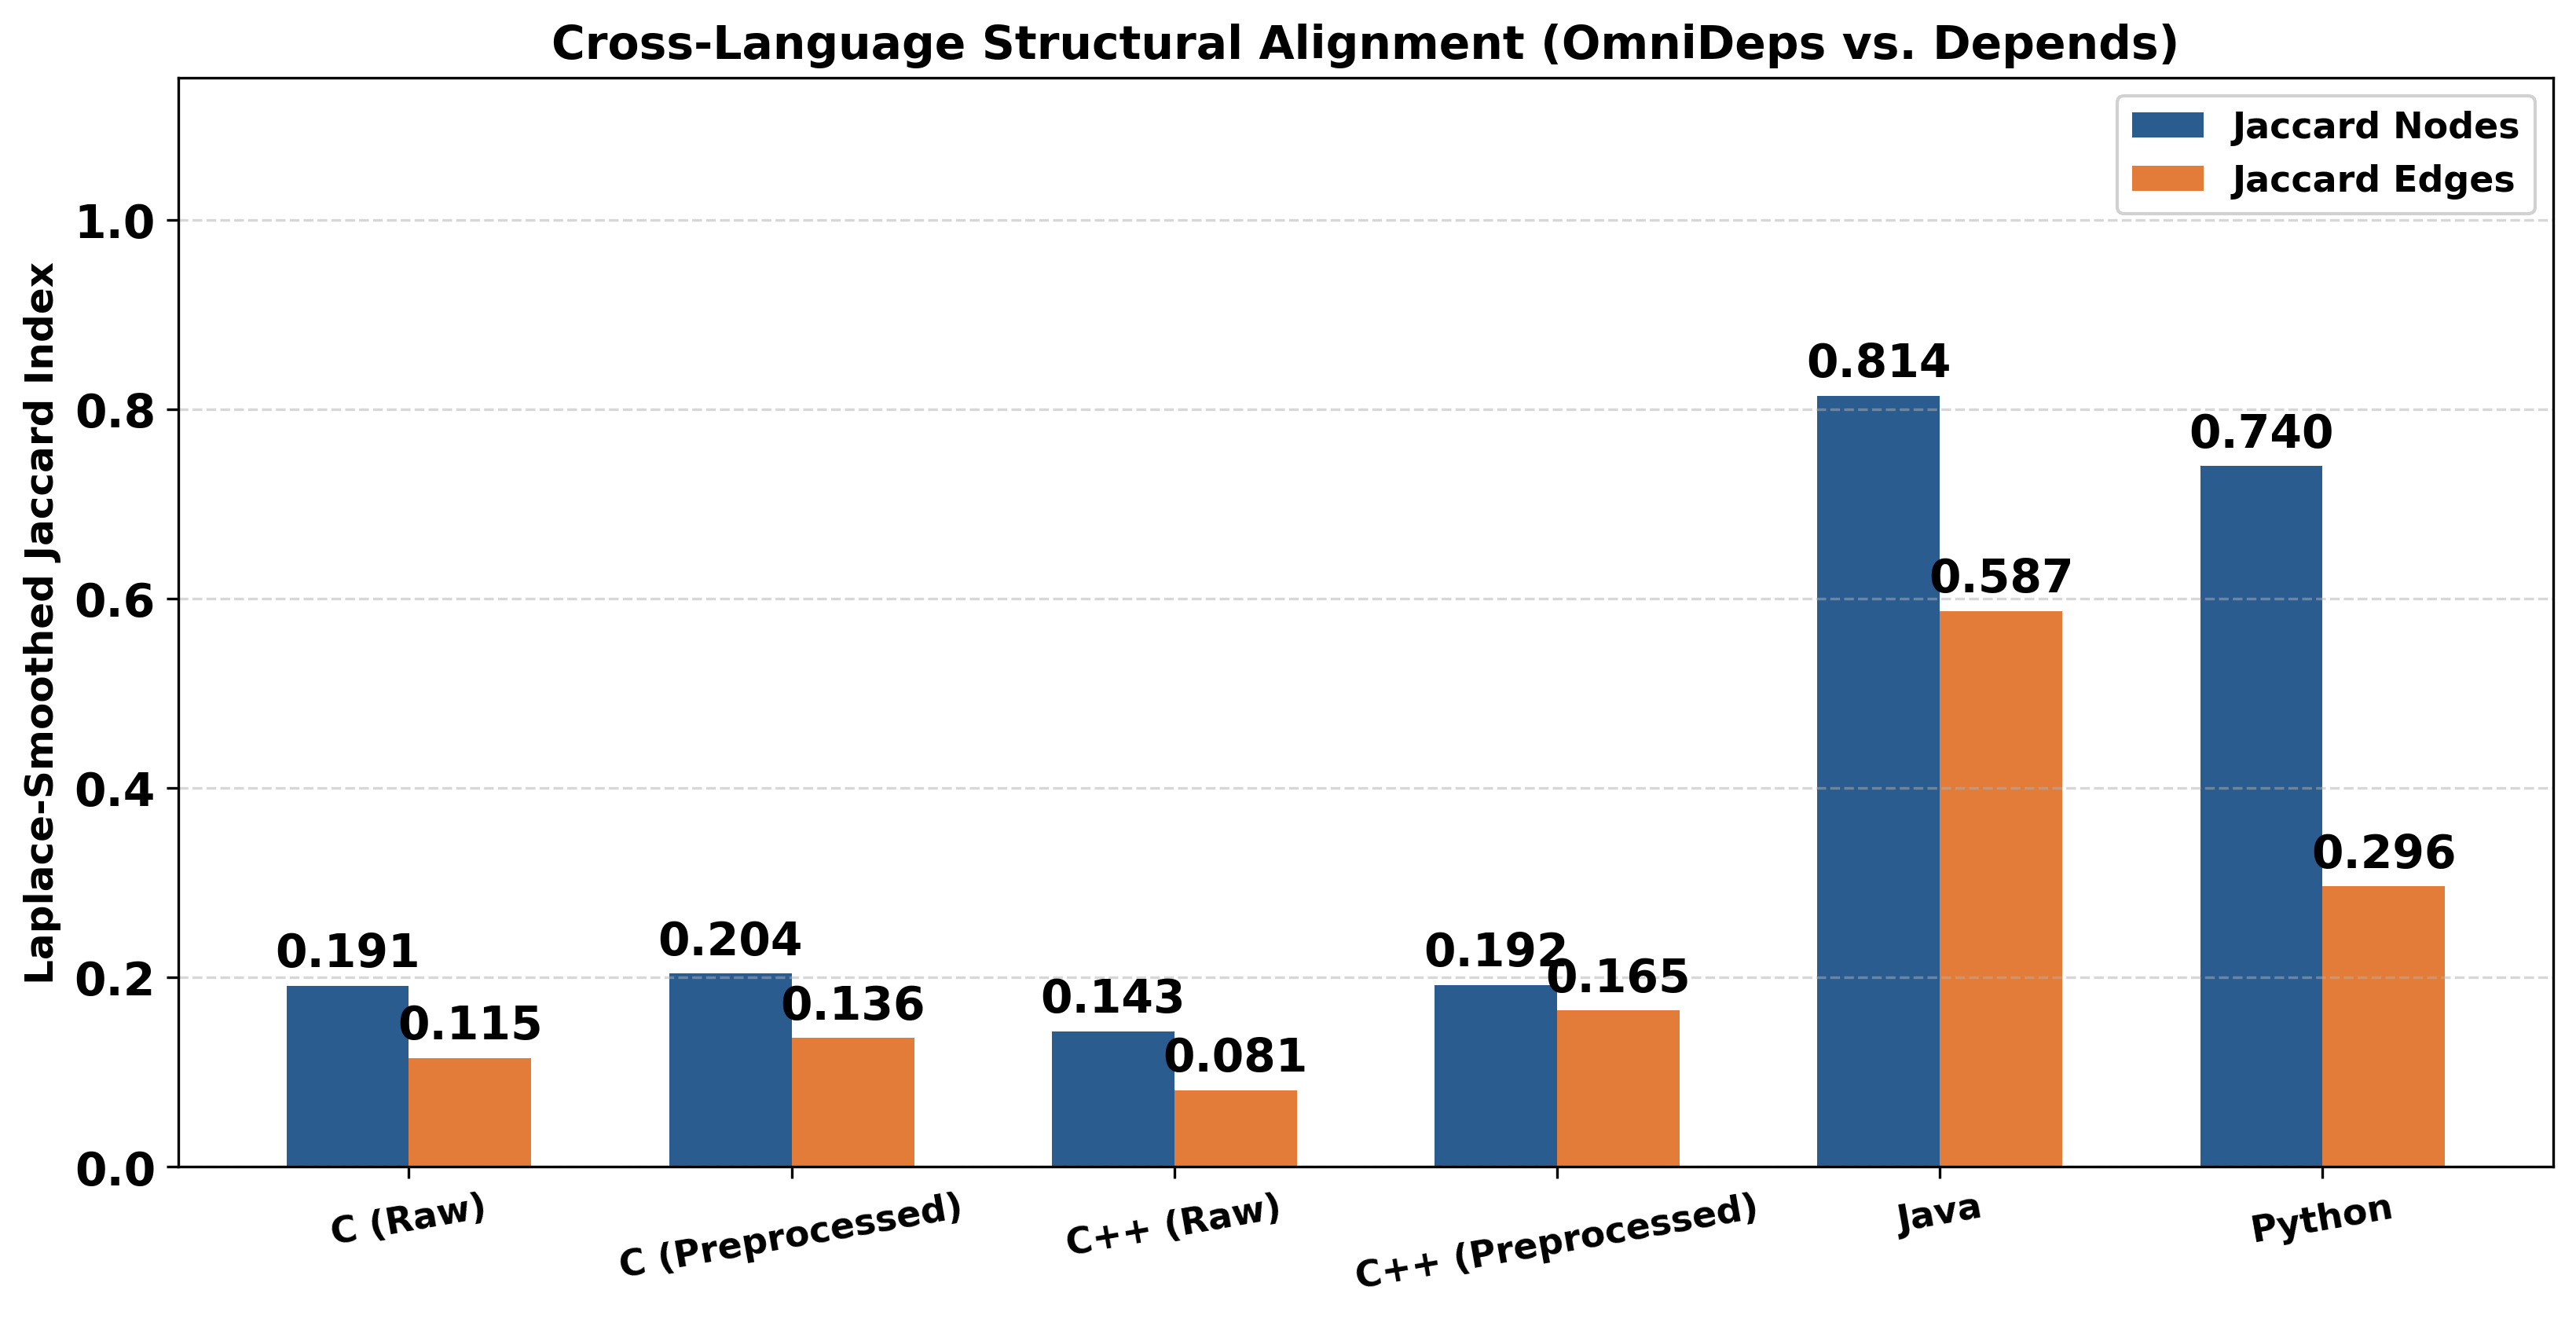
\includegraphics[width=0.98\linewidth,height=0.74\textheight,keepaspectratio]{../images/evaluation/comparisons/summary-jaccard-cross-language.png}\par
  \vspace{0.2em}
  {\scriptsize\color{cookieMuted}Mean Laplace-smoothed Jaccard similarity for nodes and edges across all comparative tool pairs\par}
\end{frame}

% BACKUP SLIDE 2: Full Empirical Agreement Matrix (Table 9.3)
\begin{frame}[noframenumbering]{Appendix: Pairwise Agreement \& Discrepancy Matrix}{Full Cross-Tool Evaluation Results Across All Comparators ($N=156$)}
  \centering
  \vspace{-0.2em}
  {\scriptsize
  \begin{tabular*}{\linewidth}{@{\extracolsep{\fill}}lccccccr@{}}
    \toprule
    \textbf{Target Pair} & $N$ & $\mathbf{J_{\text{nodes}}}$ & $\mathbf{\text{Sup}_{\text{n}}}$ & $\mathbf{\text{Inf}_{\text{n}}}$ & $\mathbf{J_{\text{edges}}}$ & $\mathbf{\text{Sup}_{\text{e}}}$ & $\mathbf{\text{Inf}_{\text{e}}}$ \\
    \midrule
    \textbf{Java} (vs. Depends)       & 31 & 0.814 (0.849) & 0.286  & 0.021  & 0.587 (0.609) & 0.406  & 0.345 \\
    \textbf{Java} (vs. Entangle)      & 19 & 0.770 (0.782) & 0.199  & 0.196  & 0.600 (0.598) & 0.359  & 0.366 \\
    \textbf{Java} (vs. Arcan)         & 18 & 0.630 (0.693) & 0.796  & 0.003  & 0.580 (0.575) & 0.759  & 0.092 \\
    \midrule
    \textbf{Python} (vs. Depends)     & 29 & 0.852 (0.882) & 0.161  & 0.048  & 0.323 (0.300) & 1.474  & 0.805 \\
    \textbf{Python} (No Imports)      & 29 & 0.852 (0.882) & 0.161  & 0.048  & 0.368 (0.387) & 1.017  & 0.834 \\
    \midrule
    \textbf{C Raw} (vs. Depends)      & 30 & 0.191 (0.167) & 14.017 & 0.619  & 0.115 (0.042) & 44.307 & 1.636 \\
    \textbf{C Preproc} (vs. Depends)  & 31 & 0.204 (0.158) & 7.218  & 0.733  & 0.136 (0.083) & 37.777 & 3.993 \\
    \textbf{C++ Raw} (vs. Depends)    & 25 & 0.143 (0.127) & 12.493 & 2.969  & 0.081 (0.039) & 58.836 & 4.769 \\
    \textbf{C++ Preproc} (vs. Depends)& 22 & 0.192 (0.151) & 4.911  & 3.229  & 0.165 (0.083) & 9.962  & 8.320 \\
    \bottomrule
  \end{tabular*}}\par
  \vspace{0.4em}
  {\tiny\color{cookieMuted}Values report arithmetic means (medians in parentheses). $\text{Sup} = |A \setminus B| / |A \cap B|$, $\text{Inf} = |B \setminus A| / |A \cap B|$. Arcan in C/C++ omitted due to ontological disparity (file vs. type).\par}
\end{frame}

% BACKUP SLIDE 3: Categorical Edge Discrepancy Breakdown (Tables 9.4 & 9.5)
\begin{frame}[noframenumbering]{Appendix: Categorical Edge Discrepancy Breakdown}{Detailed Directional Discrepancy Rates Across Dependency Kinds}
  \begin{columns}[T,onlytextwidth]
    \column{0.52\textwidth}
      \cookiekicker{Java: OmniDeps vs. Depends \& Arcan}\par\vspace{0.15em}
      {\scriptsize
      \begin{tabular*}{\linewidth}{@{\extracolsep{\fill}}lrrrr@{}}
        \toprule
        \textbf{Relation} & \multicolumn{2}{c}{\textbf{vs. Depends}} & \multicolumn{2}{c}{\textbf{vs. Arcan}} \\
        & $\Delta_{A \setminus B}$ & $\Delta_{B \setminus A}$ & $\Delta_{A \setminus B}$ & $\Delta_{B \setminus A}$ \\
        \midrule
        \texttt{belongsTo}          & 17.0\% & \textbf{1.8\%} & 36.7\% & \textbf{0.3\%} \\
        \texttt{isChildOf}          & 24.9\% & \textbf{8.7\%} & 61.3\% & \textbf{2.4\%} \\
        \texttt{dependsOn}          & 26.1\% & 26.1\%         & 43.4\% & 29.9\%         \\
        \bottomrule
      \end{tabular*}}\par
      \vspace{0.3em}
      {\tiny\color{cookieMuted}Shared edges $|A \cap B|$: \texttt{belongsTo} (6,419.1 / 3,295.7), \texttt{dependsOn} (27,890.7 / 11,374.1).\par}

    \column{0.46\textwidth}
      \cookiekicker{Python: OmniDeps vs. Depends}\par\vspace{0.15em}
      {\scriptsize
      \begin{tabular*}{\linewidth}{@{\extracolsep{\fill}}lrrr@{}}
        \toprule
        \textbf{Relation} & \textbf{Shared} & $\Delta_{A \setminus B}$ & $\Delta_{B \setminus A}$ \\
        \midrule
        \texttt{belongsTo} & 1,415.1 & 10.9\% & \textbf{4.4\%} \\
        \texttt{isChildOf} &   246.9 & 39.0\% & \textbf{22.2\%} \\
        \texttt{dependsOn} &   629.2 & 72.7\% & 72.2\% \\
        \texttt{includes}  &     0.1 & 100.0\%& 61.1\% \\
        \bottomrule
      \end{tabular*}}\par
      \vspace{0.3em}
      {\tiny\color{cookieMuted}Directional discrepancy: $\Delta_{A \setminus B} = |E_A \setminus E_B| / |E_A|$, $\Delta_{B \setminus A} = |E_B \setminus E_A| / |E_B|$.\par}
  \end{columns}
\end{frame}

% BACKUP SLIDE 4: Multi-Language Runtime Scalability (2x2 grid of log plots)
\begin{frame}[noframenumbering]{Appendix: Multi-Language Runtime Scalability}{Wall-Clock Extraction Time vs. Codebase Size (LOC) on Semi-Log Scale}
  \centering
  \begin{columns}[c,onlytextwidth]
    \column{0.50\textwidth}
      \centering
      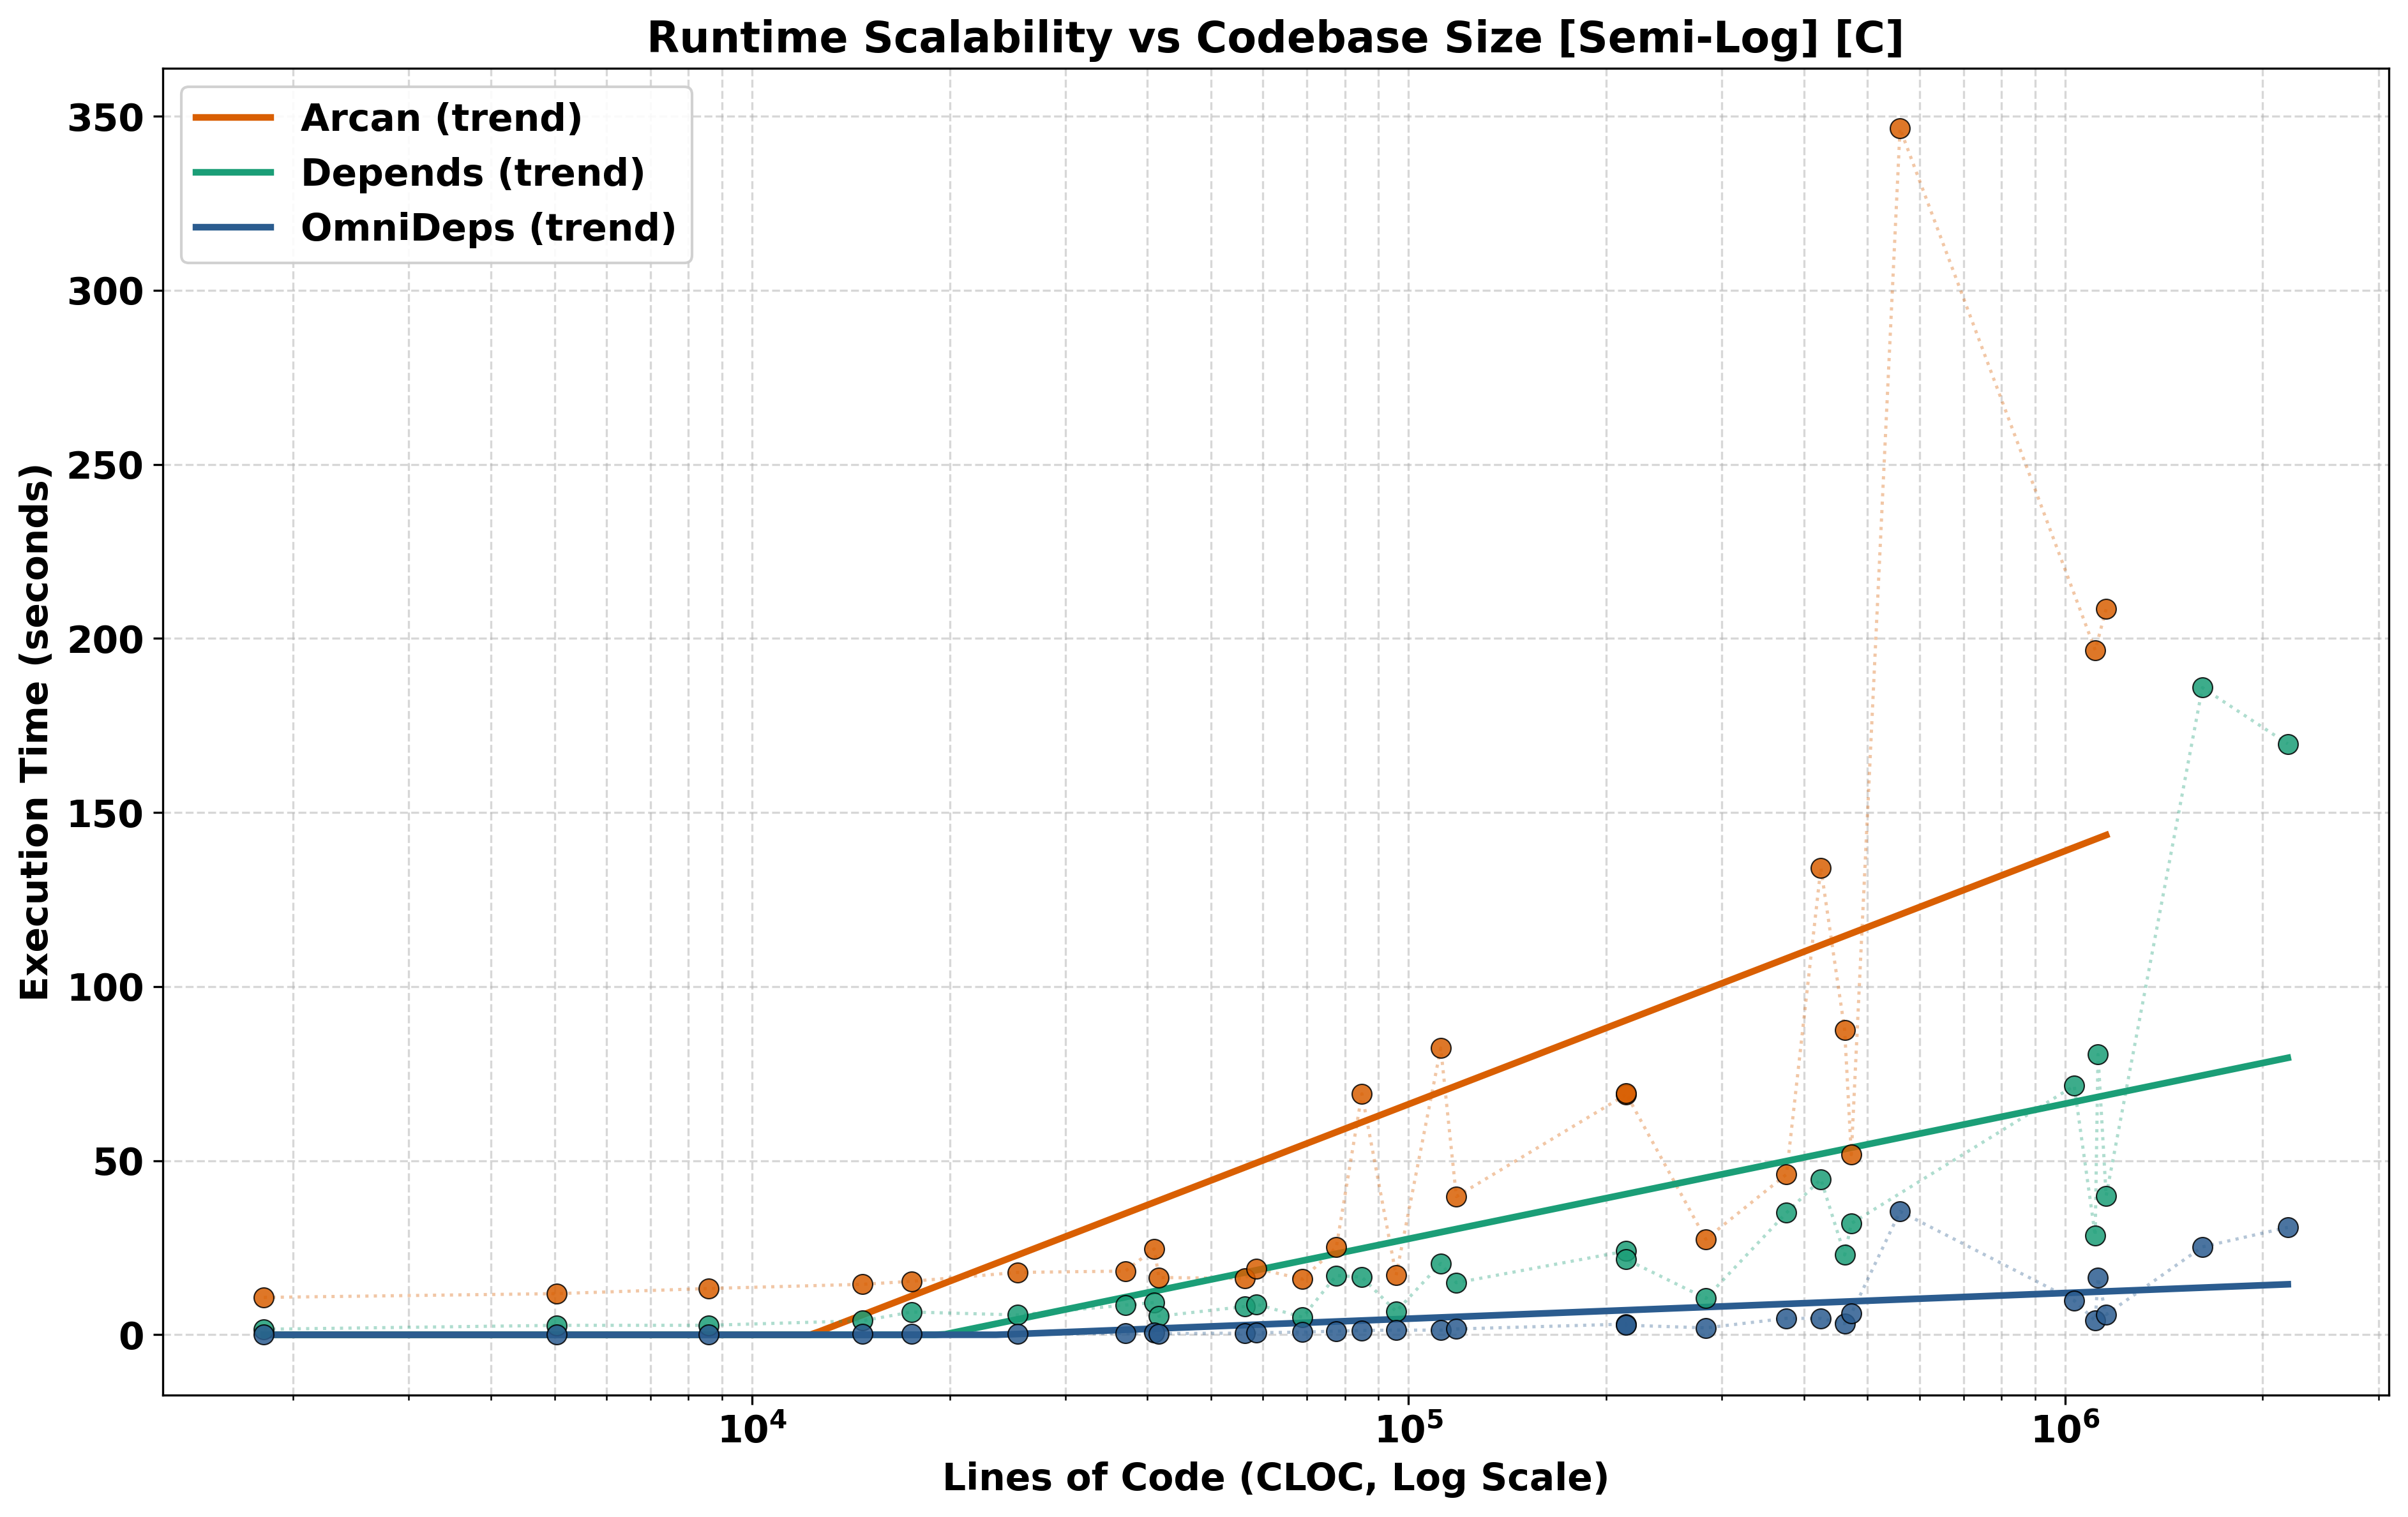
\includegraphics[width=0.96\linewidth,height=0.36\textheight,keepaspectratio]{../images/evaluation/times/graph-cloc-log-c.png}\par
      \vspace{0.3em}
      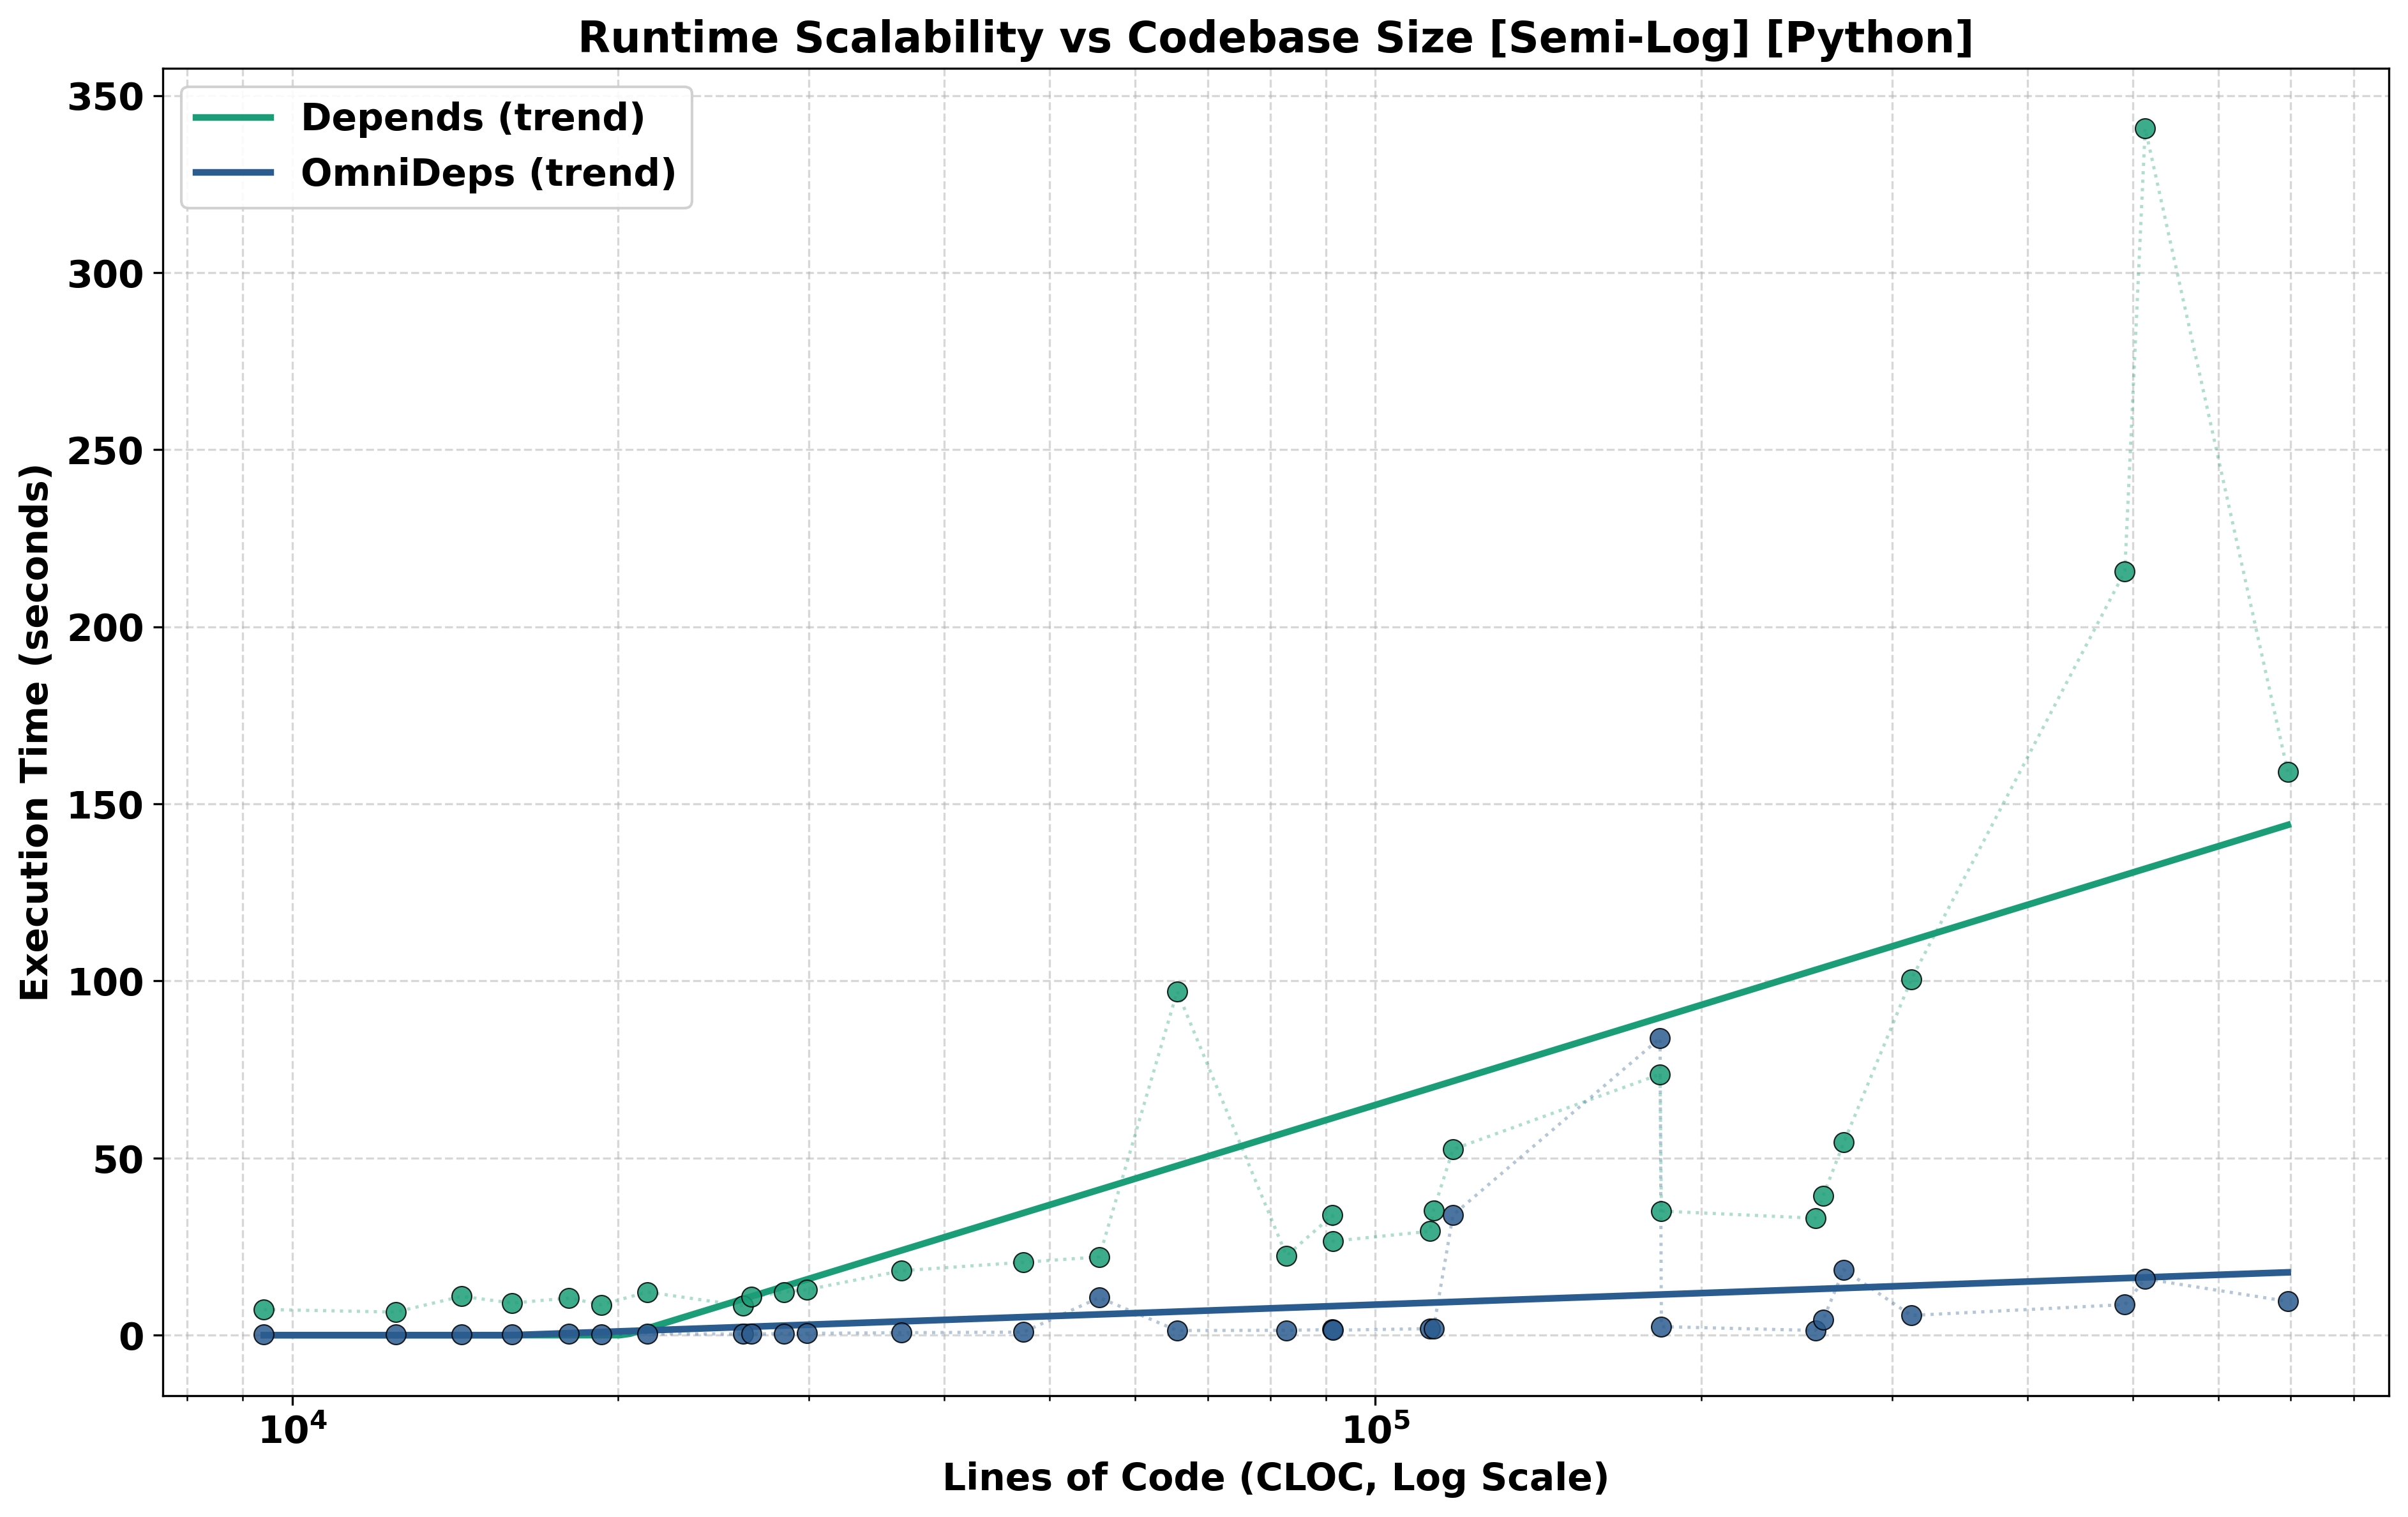
\includegraphics[width=0.96\linewidth,height=0.36\textheight,keepaspectratio]{../images/evaluation/times/graph-cloc-log-python.png}
    \column{0.50\textwidth}
      \centering
      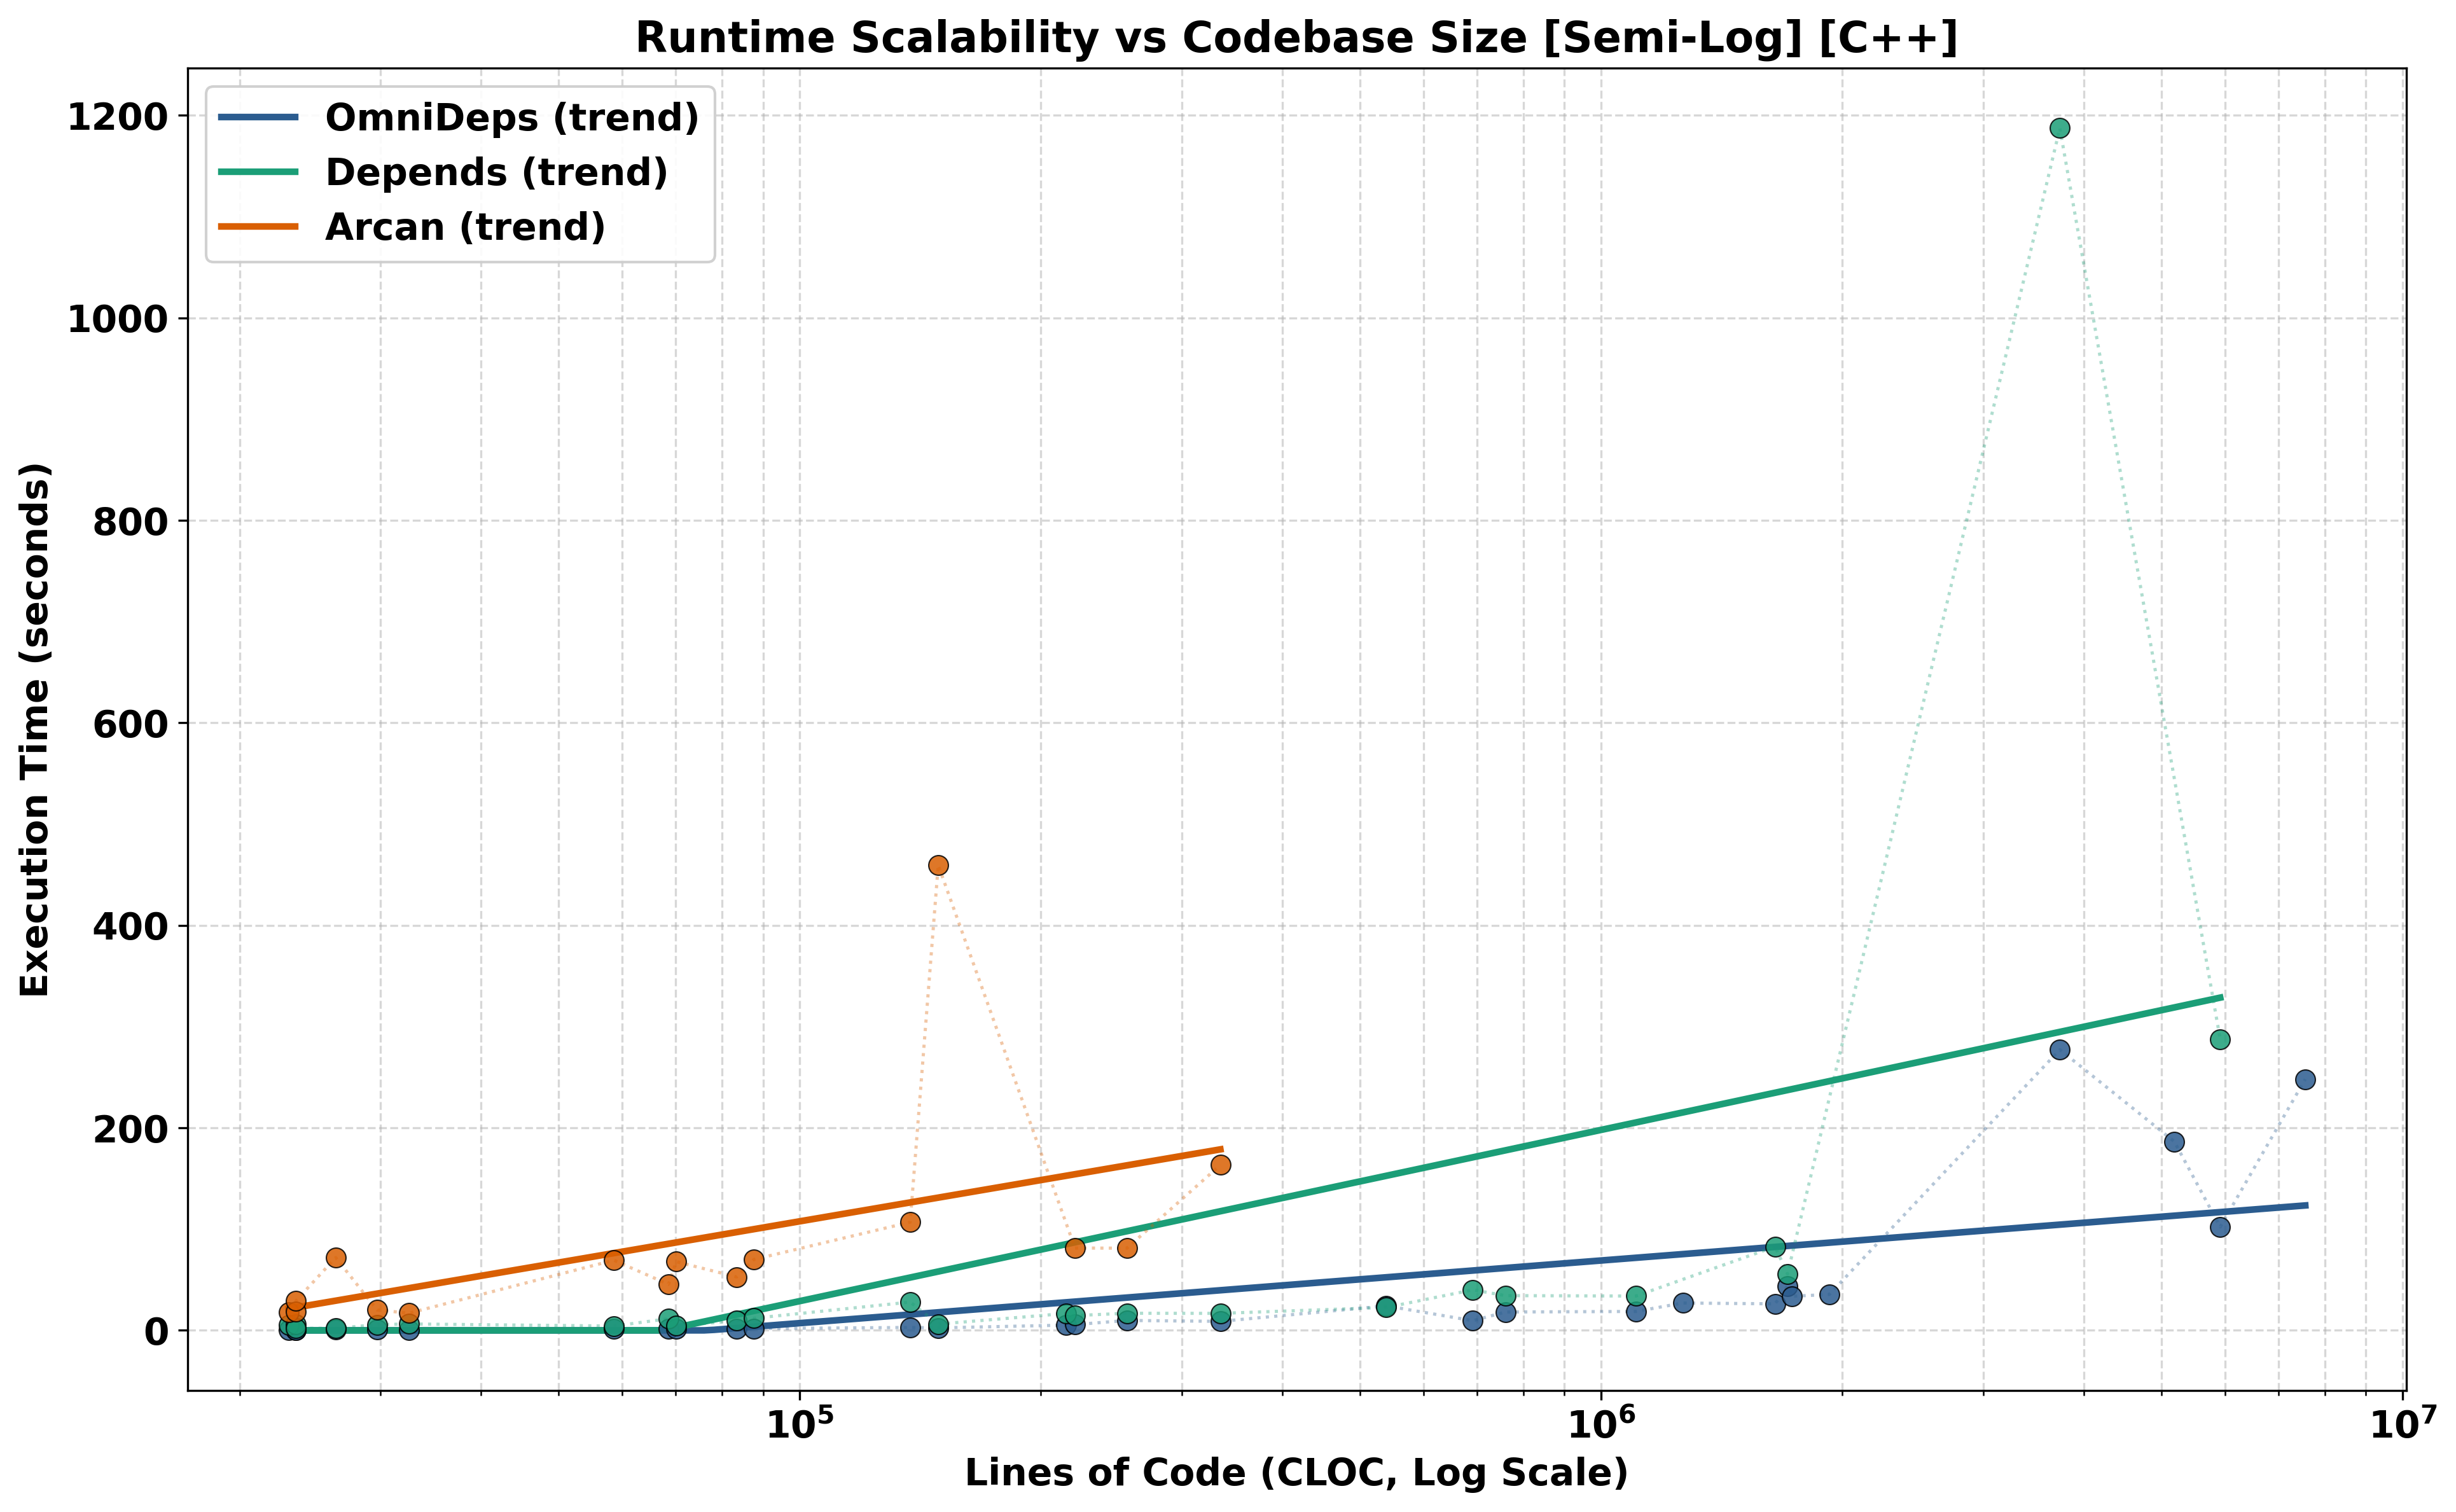
\includegraphics[width=0.96\linewidth,height=0.36\textheight,keepaspectratio]{../images/evaluation/times/graph-cloc-log-c++.png}\par
      \vspace{0.3em}
      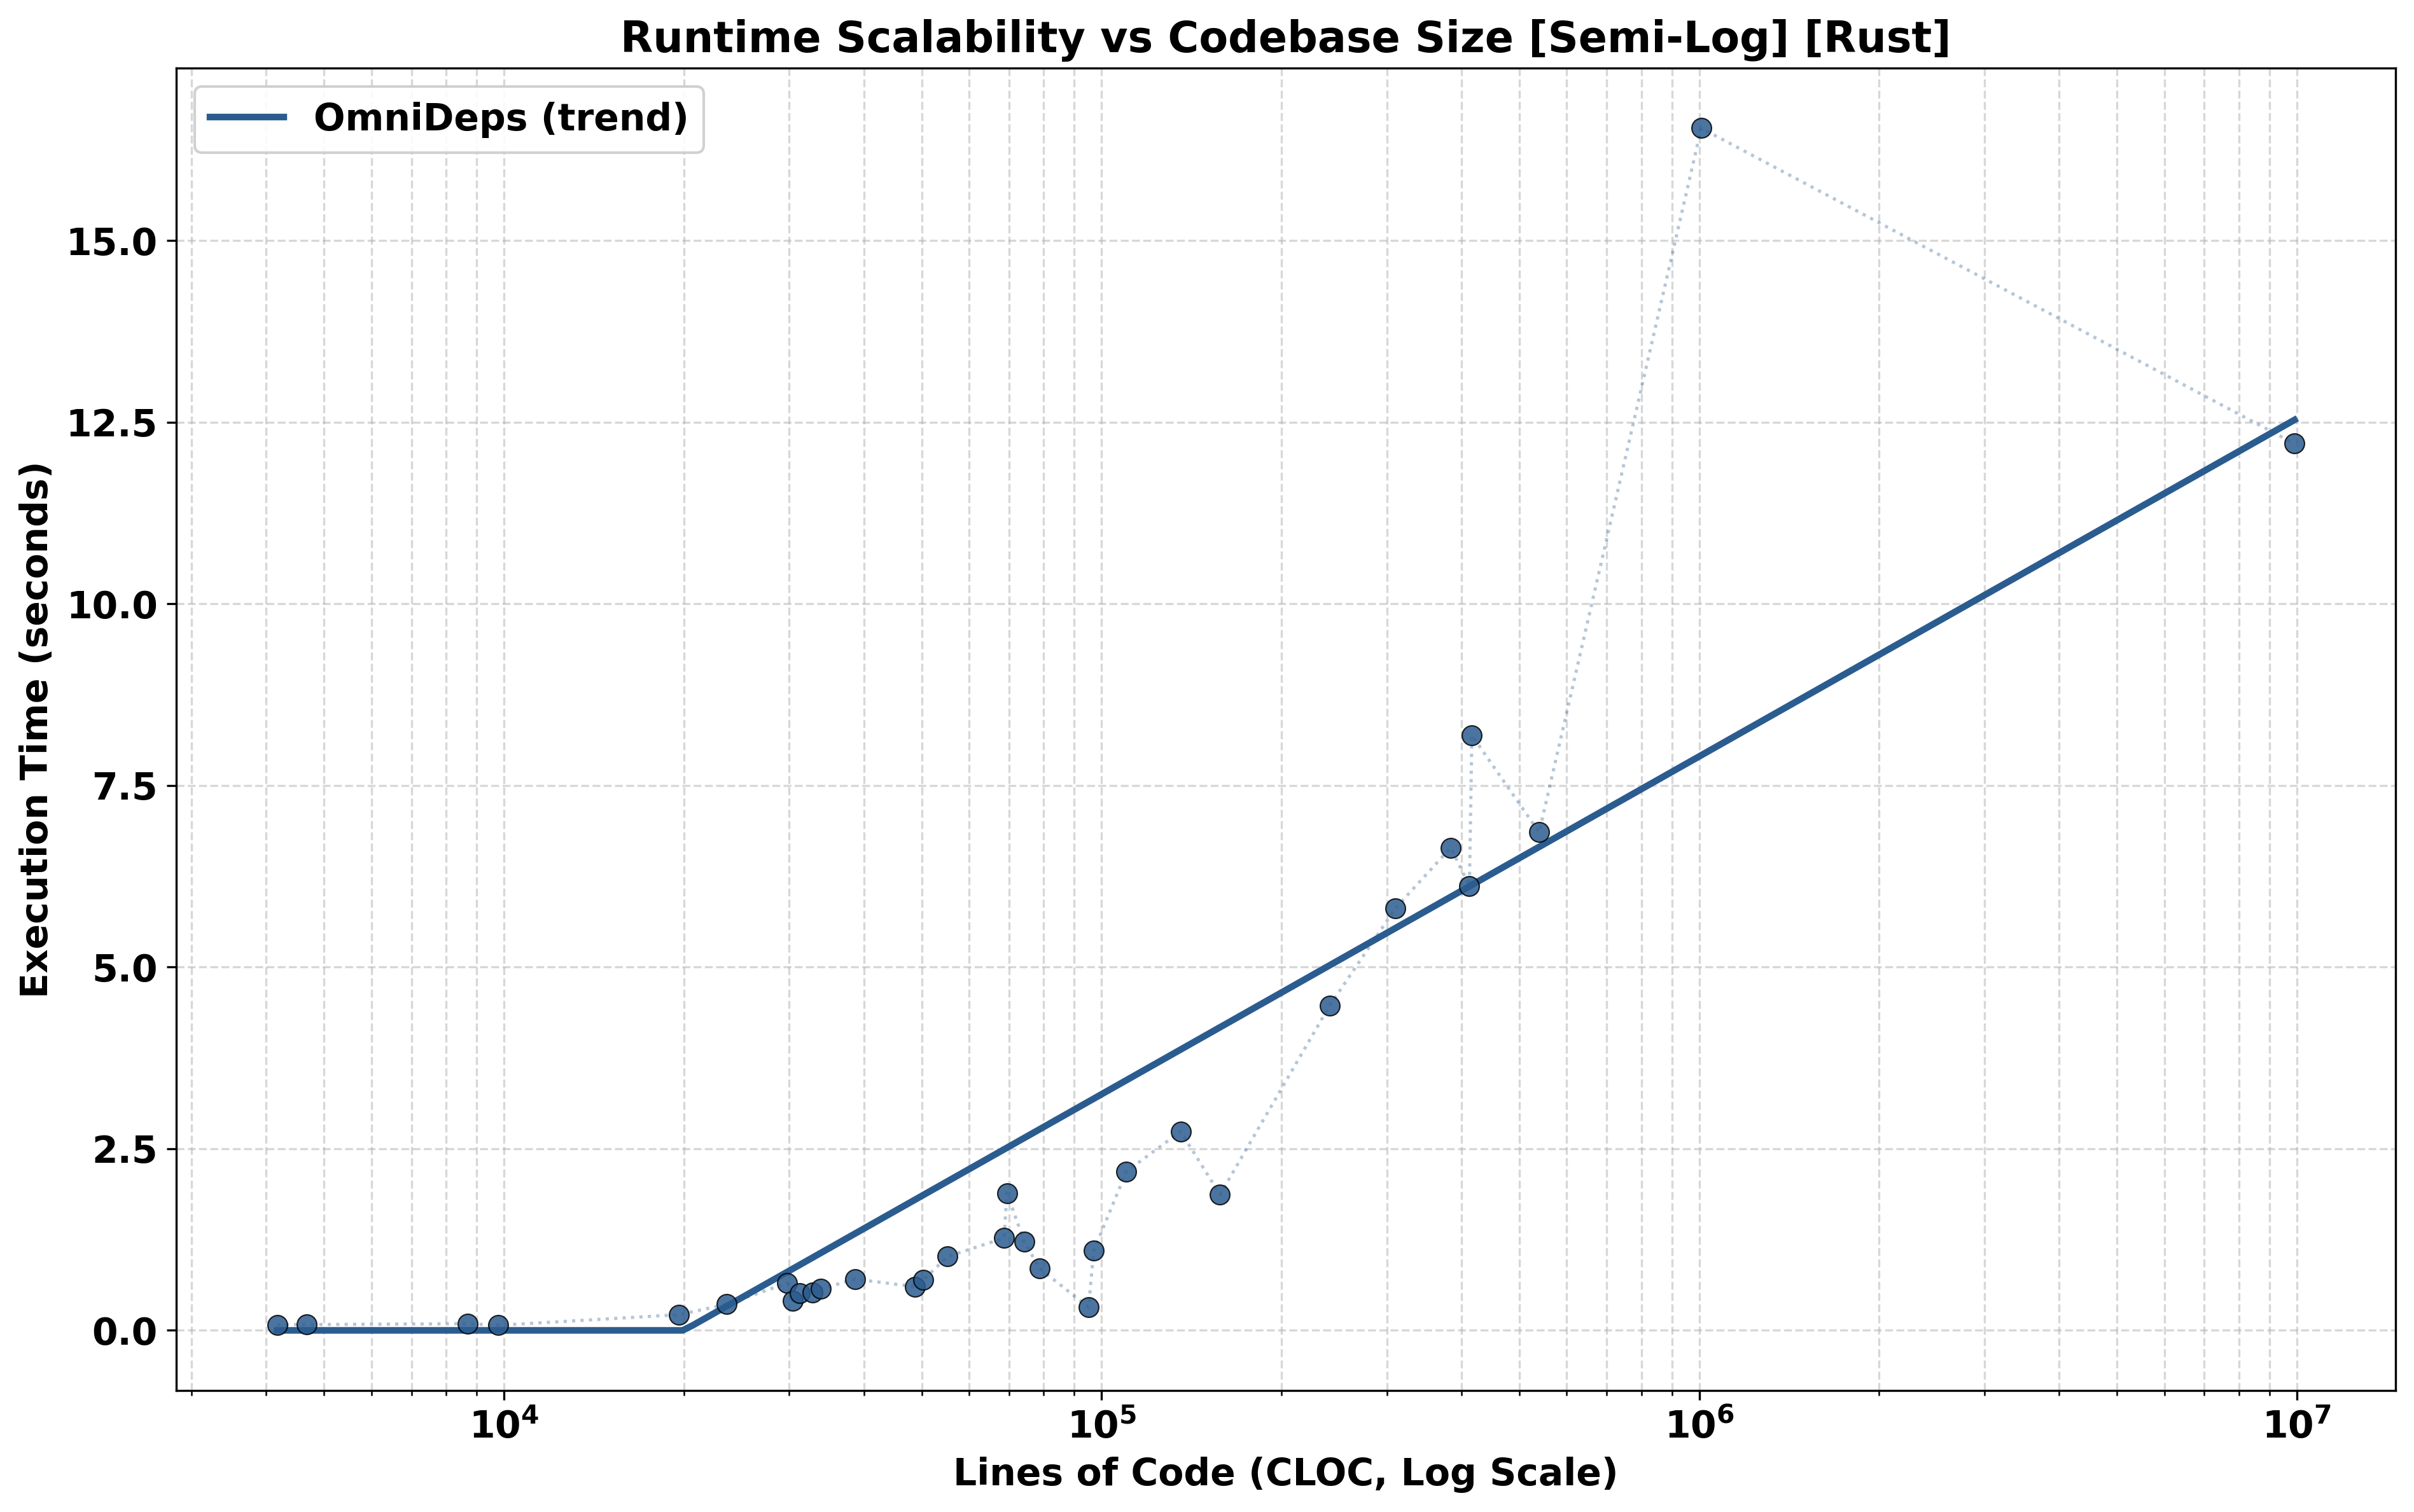
\includegraphics[width=0.96\linewidth,height=0.36\textheight,keepaspectratio]{../images/evaluation/times/graph-cloc-log-rust.png}
  \end{columns}
\end{frame}

% BACKUP SLIDE 5: Dataset Distributions (LOC & Files)
\begin{frame}[noframenumbering]{Appendix: Dataset Distributions}{Code Density (LOC/Files) and Pure Codebase Size (CLOC) across 156 Repositories}
  \begin{columns}[c,onlytextwidth]
    \column{0.50\textwidth}
      \centering
      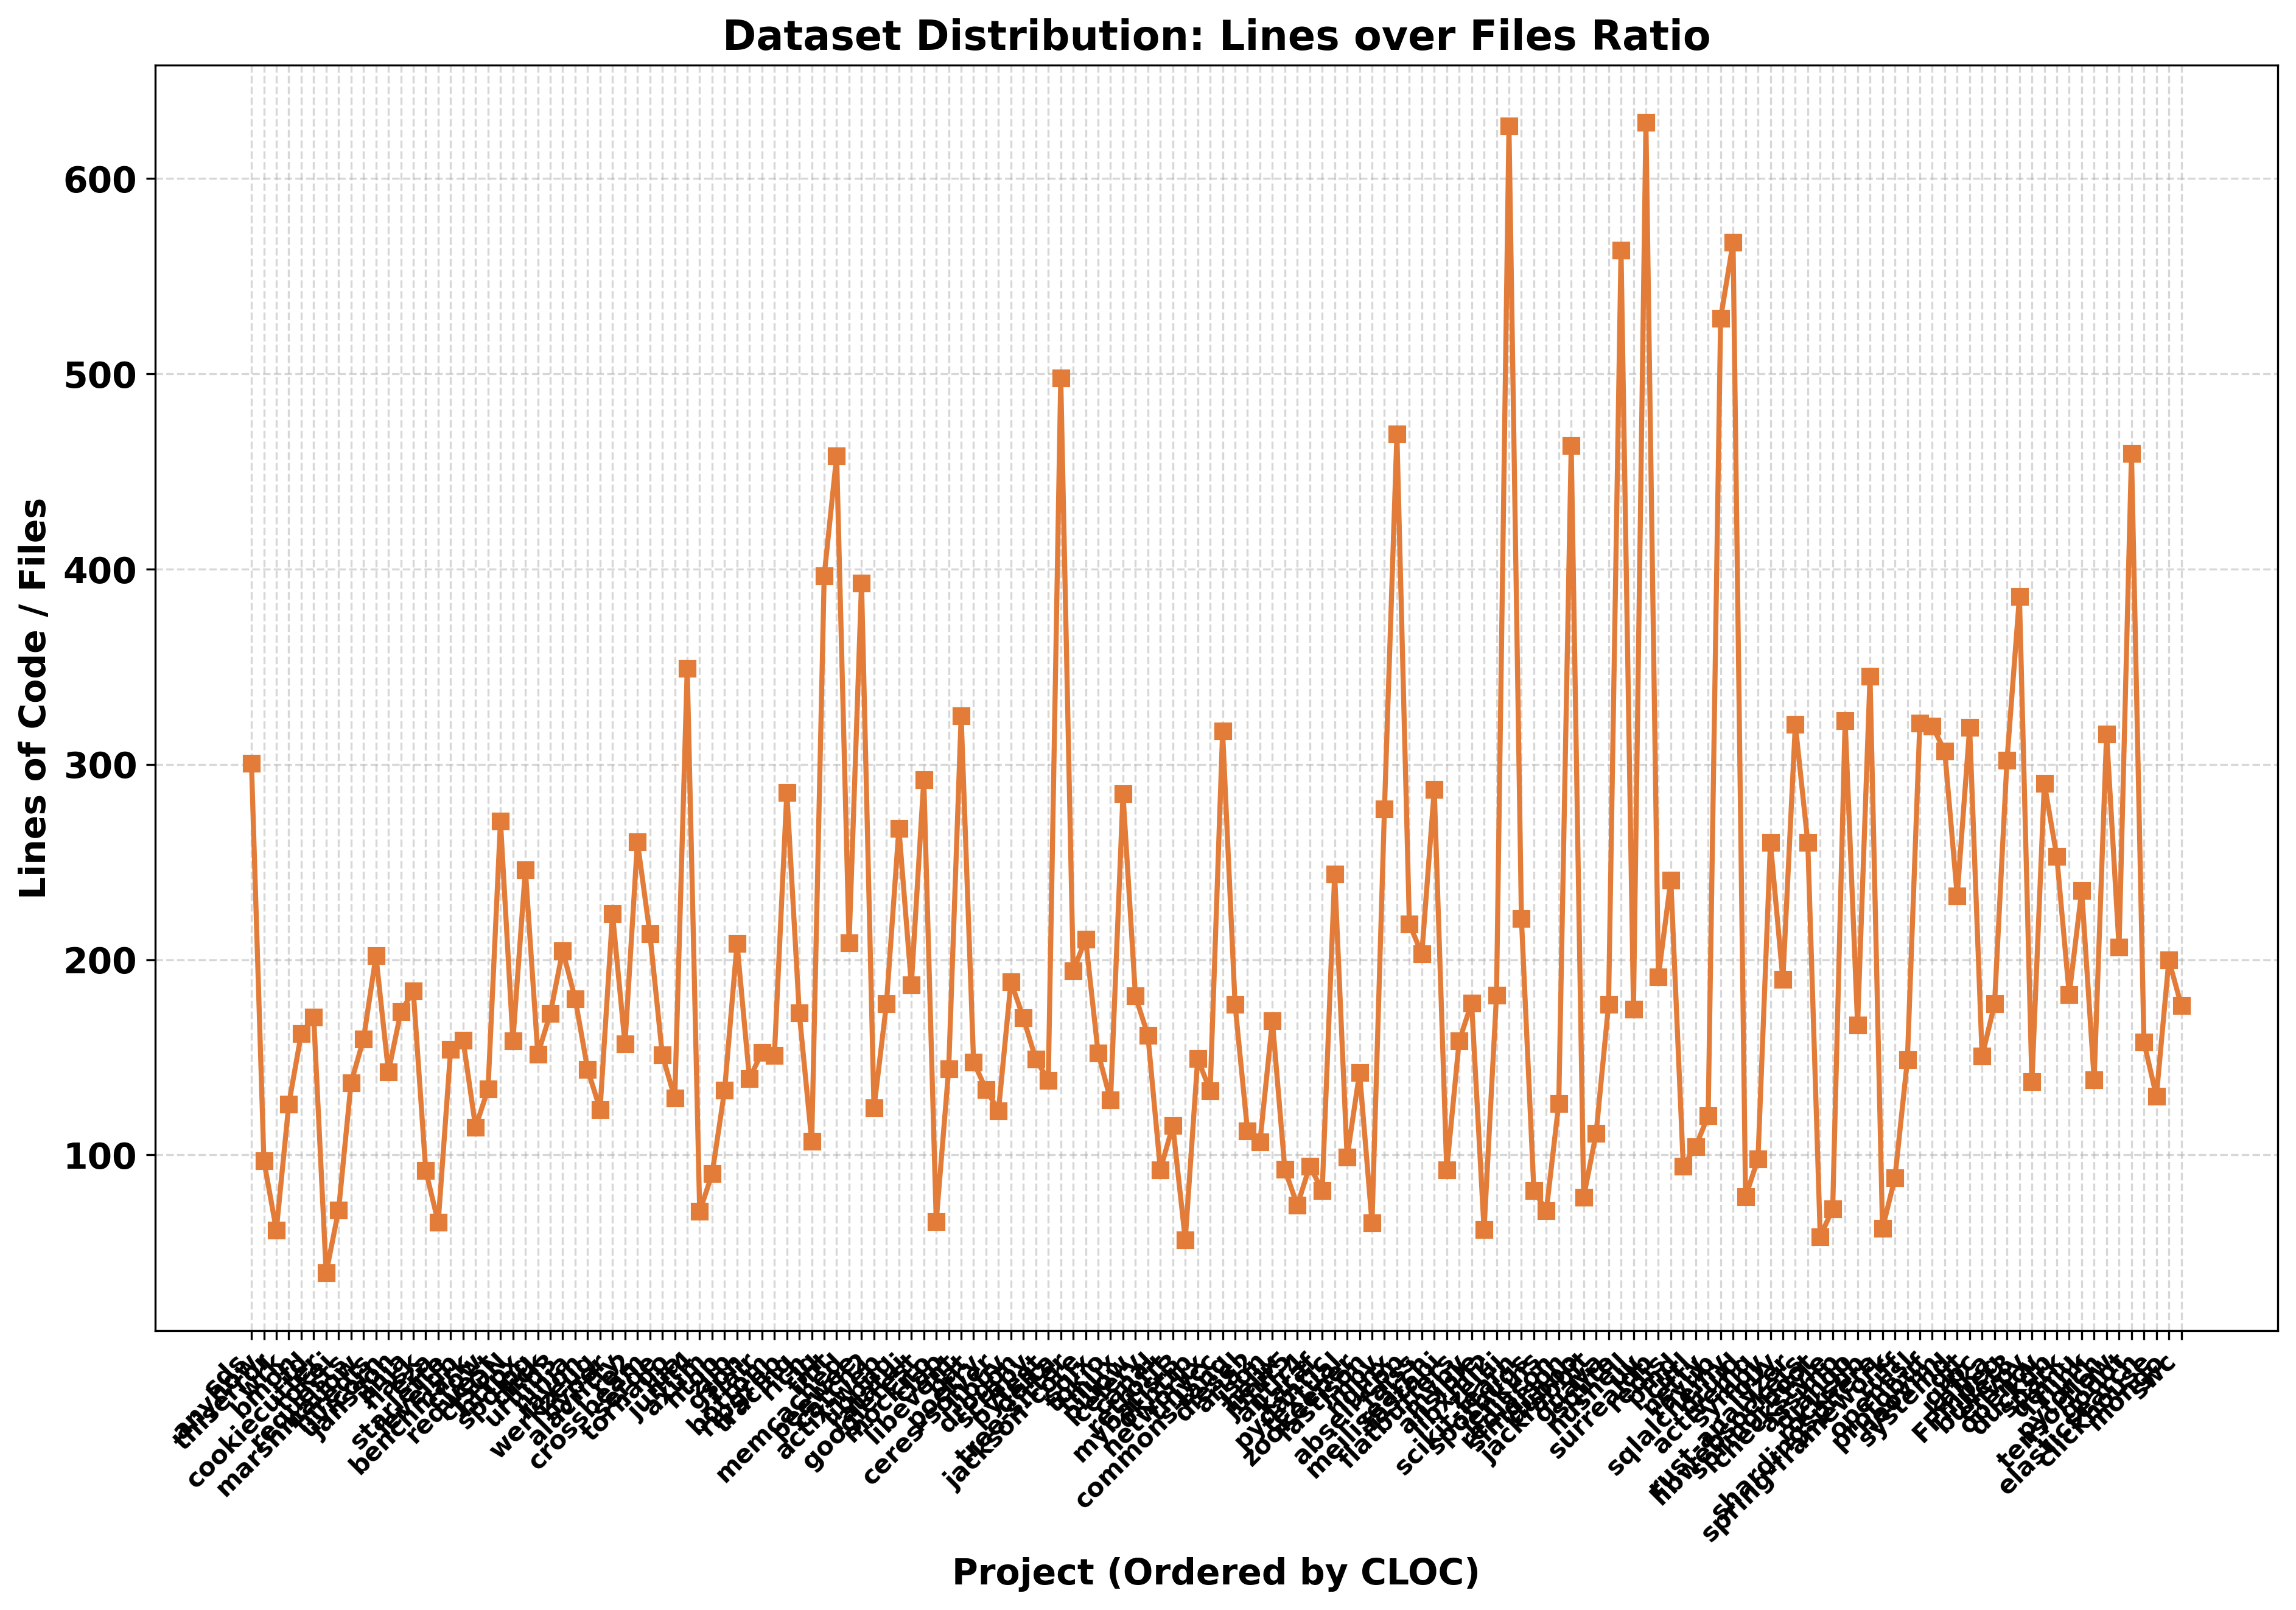
\includegraphics[width=\linewidth,height=0.72\textheight,keepaspectratio]{../images/evaluation/dataset/projects-lof.png}\par
      \vspace{0.2em}
      {\scriptsize\color{cookieMuted}Code density: Lines of Code over Files ratio\par}
    \column{0.50\textwidth}
      \centering
      \includegraphics[width=\linewidth,height=0.72\textheight,keepaspectratio]{../images/evaluation/dataset/projects-cloc.png}\par
      \vspace{0.2em}
      {\scriptsize\color{cookieMuted}Pure codebase size: Lines of Code (CLOC) ordered ascending\par}
  \end{columns}
\end{frame}

\end{document}
